\documentclass[a4paper]{report}
\usepackage[utf8]{inputenc}
\usepackage{amssymb}
\usepackage{amsmath}
\usepackage{amsthm} 
\usepackage{url}
\usepackage{xspace}
\usepackage{graphicx}
\usepackage[vlined]{algorithm2e} % lib for pseudo code
\usepackage{float}  % lib for pseudo code
\usepackage[T1]{fontenc}
\usepackage{pgfplots}
\usepackage{caption}
\usepackage{subcaption}
\usepackage{array}
\usepackage{mdframed}

\RestyleAlgo{boxruled}
\LinesNumbered


\newcolumntype{L}[1]{>{\raggedright\let\newline\\\arraybackslash\hspace{0pt}}m{#1}}

\graphicspath{ {Graphics/Images/} }

\usepackage{newunicodechar}
\newunicodechar{∙}{\cdotp}

\newcommand{\parahead}[1]{{\vspace*{6pt}\noindent\textbf{#1}\xspace\xspace\xspace\xspace}}

\newcommand{\heading}[1]{{\vspace{6pt}\noindent\sc{#1}}}

% Command for making <--> arrow with text above
\makeatletter
\newcommand\xleftrightarrow[2][]{%
  \ext@arrow 9999{\longleftrightarrowfill@}{#1}{#2}}
\newcommand\longleftrightarrowfill@{%
  \arrowfill@\leftarrow\relbar\rightarrow}
\makeatother

%\newcommand{\vectorbound}{\ensuremath{\kappa}}
%\newcommand{\secretbound}{\ensuremath{\nu}}
%\newcommand{\shortvec}[1]{\tilde{\mathbf{#1}}\xspace}
%\renewcommand{\vec}[1]{\mathbf{#1}\xspace}
%\newcommand{\cemph}[1]{\color{yellow9}{\bf #1}\xspace}
%\newcommand{\chig}{\ensuremath{\chi_{\alpha,q}}}
%\newcommand{\Ldis}{L_{\mathbf{s},\chi}^{(n)}\xspace}
%\newcommand{\sample}{\ensuremath{\leftarrow_{\$}}}
%\newcommand{\round}[1]{\ensuremath{\left\lfloor{#1}\right\rceil}\xspace}
%\newcommand{\Bdis}[1]{B_{\mathbf{s},\chi}(b,#1,p)\xspace}
%\newcommand{\Bdissm}[1]{B_{small,\mathbf{s},\chi}(b,#1,p)\xspace}
%\newcommand{\svec}{\ensuremath{\mathbf{s}}\xspace} % command for pseudo code
%\newmdtheoremenv[frametitlerule=true, frametitlebackgroundcolor=gray!20]{defi}
%\newcommand{\E}{\ensuremath{\textnormal{E}}}
%\newcommand{\Var}{\ensuremath{\textnormal{Var}}}
%\newcommand{\U}[1]{\ensuremath{\mathcal{U}(#1)\xspace}}
%\newcommand{\abs}[1]{\ensuremath{|#1|}\xspace}


\newcommand{\dotp}[2]{\ensuremath{\left\langle {#1},{#2}\right\rangle}\xspace}
\newcommand{\Z}{\ensuremath{\mathbb{Z}}\xspace}
\newcommand{\Zq}{\ensuremath{\Z_q}\xspace}
\newcommand{\ZqStar}{\ensuremath{\Z_q^*}\xspace}
\newcommand{\Zp}{\ensuremath{\mathbb{Z}_p}\xspace}

\def\polyfactor{n\, \log_2^2 n}
\newcommand{\bigO}[1]{\ensuremath{\mathcal{O}\left(#1\right)}\xspace}
\renewcommand{\O}[1]{\ensuremath{{\mathcal{O}\left(#1\right)}}\xspace}


\theoremstyle{plain}
\newtheorem{thm}{Theorem}[subsection]
\newtheorem{lemma}{Lemma}[subsection]

\mdfdefinestyle{defstyle}{frametitlerule=true, frametitlerulewidth=0px}
\mdtheorem[style=defstyle]{defi}{Definition}[subsection]

\mdtheorem[style=defstyle]{infobox}{}[subsection]

\begin{document}

%***************************************************************
%               Title Page
%***************************************************************
\begin{titlepage}

\newcommand{\HRule}{\rule{\linewidth}{0.5mm}} % Defines a new command for the horizontal lines, change thickness here

\center % Center everything on the page
 
%----------------------------------------------------------------------------------------
%	HEADING SECTIONS
%----------------------------------------------------------------------------------------

\textsc{\LARGE Aalborg university}\\[1.5cm] % Name of your university/college
\textsc{\Large Master of IT, Software Development}\\[0.5cm] % Major Heading
\textsc{\large Master thesis}\\[0.5cm] %Minor Heading 

%----------------------------------------------------------------------------------------
%	TITLE SECTION
%----------------------------------------------------------------------------------------

\HRule \\[0.4cm]
{ \huge \bfseries Electronic voting application based on public verifiable secret sharing}\\[0.4cm] % Title
\HRule \\[1.5cm]
 
%----------------------------------------------------------------------------------------
%	AUTHOR SECTION
%----------------------------------------------------------------------------------------

\begin{minipage}{0.4\textwidth}
\begin{flushleft} \large
\emph{Author:}\\
Sune Chung \textsc{Jepsen} % Your name
Kasper Jensen \textsc{Lemming} % Your name
\end{flushleft}
\end{minipage}
~
\begin{minipage}{0.4\textwidth}
\begin{flushright} \large
\emph{Supervisor:} \\
Ignacio \textsc{Cascudo} % Supervisor's Name
\end{flushright}
\end{minipage}\\[2cm]

% If you don't want a supervisor, uncomment the two lines below and remove the section above
%\Large \emph{Author:}\\
%John \textsc{Smith}\\[3cm] % Your name

%----------------------------------------------------------------------------------------
%	DATE SECTION
%----------------------------------------------------------------------------------------

{\large June 2017}\\[2cm] % Date, change the \today to a set date if you want to be precise

%----------------------------------------------------------------------------------------
%	LOGO SECTION
%----------------------------------------------------------------------------------------

\includegraphics{AAU_LOGO.png}\\[1cm] % Include a department/university logo - this will require the graphicx package
 
%----------------------------------------------------------------------------------------

\vfill % Fill the rest of the page with whitespace

\end{titlepage}



\chapter*{Abstract}
\input{010_abstract.tex}
\clearpage

\tableofcontents
\clearpage


%***************************************************************
%               Part 1: Introduction
%***************************************************************
\chapter{Introduction}
    \section{Introduction}
In this master thesis we will study how to implement an  electronic voting scheme application which is based on some tools from cryptography where the most important tool is the Publicly Verifiable Secret Sharing (PVSS) protocol. The main paper for this protocol will be Berry Schoenmakers paper "A Simple Publicly Verifiable Secret Sharing Scheme and its Application to Electronic Voting" \cite{Schoenmakers1999}. \\\\
\noindent
Secret sharing is a tool which used in the PVSS protocol. Secret sharing is a way of distributing a secret among several servers. Secret sharing is where a dealer has a secret. The dealer shares pieces of the secret to each of the players. If there are a large number of players they will be able to reconstruct the secret. More technically the idea is to hide a secret inside of a polynomial so that given certain partial information of the polynomial we can recover the secret that was hidden in it.\\\\
\noindent
A Multiparty computation protocol (MPC) is a protocol which uses secret sharing and allows several parties to compute some function on some private inputs, in such a way that they learn the result but not the inputs from the other players. MPC is not using conventional methods, where some commonly trusted party, could gather sensitive information. The figure to the left is showing a judge who all participants trust to give their secret inputs. The trusted party can then compute the outcome of the process, for instance the sum of all inputs, and reveal the output. The right figure is equivalent MPC would work. Here there is no trusted party, but by using multiparty computation they can still achieve the same level of secrecy, but without having to trust someone.
 
\begin{center}
     \makebox[\textwidth]{\includegraphics[scale=0.35]{MPC.jpg}}
\end{center}

\noindent
This leads to a core observation namely that without a trusted party the ability to validate the input the MPC protocol relies on the participants honesty. 
The PVSS protocol used in this thesis proposes a solution to this problem. The idea is that not only can the participants verify their own shares, but that anybody can verify the correctness of the transmitted data.
    
    \section{Motivation}
There are theoretical papers about how participants can communicate secure. For different reasons there are fewer papers which propose how to implement their theoretical results. This master thesis will try to combine a theoretical paper and how it actually can be implemented in a practical case. 
    
    \section{Objectives}
This project consist of two main parts. The first a theoretical background where we study the electronic voting protocol described in \cite{Schoenmakers1999}. In order to understand the protocol, some study in the basic field of cryptography is required. In the second part of the project, we will try to design and implement an application based on the protocol. Basically this master thesis have at the following objectives. 

\begin{enumerate}
    \item   Describe the theory behind secret sharing and multiparty computation as well as the cryptographically concept needed to understand it. The aim is to describe the theories clearly and with examples such that one really understands how it works. 
            
    \item   Describe the Electronic Voting Protocol \cite{Schoenmakers1999} and the mathematically justification behind it, again aiming to describe the protocol clearly and with examples to really understands how it works. 
    
    \item   Design and implement a secure and scalable electronic voting application based on the protocol. Known software design principles will be used to acquire high and reliable software quality.
    The aim is to make the application web based, given the potential of such an application.
\end{enumerate}



    
    \section{Limitations}

The following limitations have be identified.

\begin{itemize}
    \item The field of multiparty computation if broad and there exist numerous of scientific papers describing different protocol. This thesis will only focus on the main concepts in order to understand
    the electronic voting protocol. 
    
    \item Even though the aim is for high and reliable software quality, the application designed and developed in this thesis is to be considered proof-of-concept. 
\end{itemize}
    
    \section{Document Structure}
Here we present the content of the rapport. One section will contain the mathematical description of the protocol. The second section will be about the pratical part of the electronic voting application, where we will describe our implementation.


 \clearpage
%***************************************************************
%               Part 2: Voting
%***************************************************************  
\chapter{Voting}    
    \section{Overview}



\section{The Voting Process}



\section{Challenges}



\section{Security Requirements}


\clearpage
%***************************************************************
%               Part 3: Mathematical understanding
%***************************************************************
\chapter{Mathematical understanding}
    \input{110_Part_1_Protocol.tex}
    
    \section{Method}
To ensure structure the sections will be contructed based one or more of the following parts.
\begin{enumerate}
    \item General structure 
    \begin{enumerate}
        \item Informal description
        \item Definition
        \item Example
        \item Proof    
   
    \end{enumerate}
  
    \item Pseudo code
\end{enumerate}

\begin{description}
    \item[General structure] The general rule will be that every section will start informal description of the subject. Here we will give a informal description of why this it is relevant to our rapport. After that a more formal description will come. Their will be parts where the formality will require a more in depth explanation. To avoid disruption we then put this formality last in the section. 
    
    
    \item[Pseudo code]  We will use pseudocode as an informal technique to outline the structure of our algorithms. This technique aims to describe a solution so that it is easy to read for humans.

\end{description}


    
    \section{Modular arithmetic}
Modular arithmetic, is a simple way of performing arithmetic in a finite set of integers.

%**************************************Definition Modulo Operation Start
\begin{defi}[\textbf{Modulo Operation}]
Let \begin{math} a, r,m \in  \mathbb{Z}\end{math} (where \begin{math} \mathbb{Z}\end{math} is a set of all integers) and \begin{math} m > 0\end{math} and we write  
\begin{center} \begin{math} a = r \ mod \ m\end{math} \end{center}
if \begin{math}m \end{math} divides \begin{math} a - r \end{math}.\\
\begin{math}m \end{math} is called the modulus and \begin{math}r \end{math} is called the remainder.
\end{defi}
%**************************************Definition Modulo Operation End

\parahead{Computing the remainder} By example we can compute the remainder according to the definition. Given: \begin{math} a, m \in \mathbb{Z} \end{math} we compute the remainder by the following fomular:  \begin{math} a = qm +r \end{math}. This example illustrate that the remainder is not unique. Though the remainder will be unique in set $[0,$ m $)$.

\noindent
\begin{alignat*}{8}
42 &= 4 \cdot 9 +6 &&\implies r &&= 6 ,\ &&\text{by \ definition}: \  &&(42-6) &&= 36 ,  9| 36 \\
42 &= 3 \cdot 9 +15 &&\implies r &&= 15 ,\ &&\text{by \ definition}: \ &&(42-15) &&= 27 ,  9| 27 \\
42 &= 5 \cdot 9 +(-3) &&\implies r &&= -3 ,\ &&\text{by \ definition}: \ &&(42-(-3)) &&= 45 ,  9| 45 
\end{alignat*}




\parahead{Equivalence classes} Above can also be written with the modulo operator. Here we show that all have different remainder but are in the same equivalence class modulo \textit{9}. This means that all members of a given equivalence class behave equivalently. Note also that one can compute with negative integers.

\begin{align*}
42 &= 6 \ mod \ 9 \\
42 &= 15 \ mod \ 9 \\
42 &= -3 \ mod \ 9 
\end{align*}

\parahead{Computing the inverse}
As we will see later, computing the inverse becomes an important part in this protocol for how to divide modulo an integer arithmetically. For this we have the Extended Euclidean algorithm which allows us to compute the inverse modular some integers. This computation results in computing the inverse.


\parahead{Extended Euclidean algorithm} To compute the inverse means that we want to compute the following \begin{math}a\ \cdot \ x \ mod \ q = 1 \end{math} where $a, \ x, \ q$ are integers and $x$ is the inverse of $a$. The condition for the existence of the inverse is that the $gcd(q,\ a)= 1$. This means that the only number which divides both $q$ and $a$ is $1$. So if $gcd(q,\ a)= 1$ the Extended Euclidean Algorithm computes the inverse of $a$.\\


\parahead{Explanation of the Extended Euclidean algorithm (EEA)} Since we will use an implementation in our electronic voting application we will explain the EEA by example. In order to explain the EEA we will explain the regular Euclidean algorithm (EA). The first two lines (6-7) in the algorithm is the EA. It turns out that if the $gcd(n,a)=1$  and we give the EEA $gcd(n,a)$, where $n$ is the modulo integer and $a$ is an integer, then the $t$ parameter will be the inverse of $a$. 
\cite{Paar}

%**************************************Pseudocode Euclidean algorithm start
\begin{center}
\begin{algorithm}[H]
\caption{Extended Euclidean Algorithm (EEA)\label{alg}}

\SetKwRepeat{Do}{do}{while}

\KwIn{positive integers $r_0 $ and $r_1 $ with $r_0 $ > $r_1 $}
\KwOut{gcd($r_0 $, $r_1 $), as well as s and t such that gcd($r_0$, $r_1$) = $s \cdot r_0+t \cdot r_1 $.}

\textbf{Initialization:} \\
$
\begin{array}{ll}
    s_0 = 1   & t_0 = 0 \\
    s_1 = 0   & t_1 = 1 \\
      i = 1     &           \\
\end{array}                 
$

\Begin{
    \Do{$r_i \neq 0 $}{
    $i = i+1 $\\
    $r_i = r_{i-2} \ mod \ r_{i-1} $\\
    \begin{math} \mathbf{ q_{i-1} = ( r_{i-2}-r_{i} ) / r_{i-1} }  \end{math}\\
    $s_i = s_{i-2}-q_{i-1} \cdot s_{i-1} $\\
    $t_i = t_{i-2}-q_{i-1} \cdot t_{i-1} $
    }

\Return{ \\
    gcd($r_0 $, $r_1 $) = $r_{i-1} $\\
    s = $s_{i-1} $\\
    t = $t_{i-1} $
    }
}
\end{algorithm}
\end{center}


%**************************************Pseudocode Euclidean algorithm end
\noindent
The EA works that given to integers $r_0 = 911$ and $r_1 = 301$. The gcd is computed by reducing the problem of finding the gcd of two given numbers to that of the gcd of two smaller numbers 


\begin{center}
\begin{tabular}{|ll|lll| } 
\hline
$911$ & $= 3 \cdot 301 +8$& $gcd(911,301)$ & $= gcd(301,8)$ & \\ 
\hline
$301$ & $= 37 \cdot 8+5$ & $gcd(301,8)$ & $= gcd(8,5)$ &\\ 
\hline
$8$ & $= 1 \cdot 5+3$ & $gcd(8,5)$ & $= gcd(5,3)$ & \\ 
\hline
$5$ & $= 1 \cdot 3+2$ & $gcd(5,3)$ & $= gcd(3,2)$ & \\ 
\hline
$3$ & $= 1 \cdot 2+1$ & $gcd(3,2)$ & $= gcd(2,1)$ & \\ 
\hline
$2$ & $= 1 \cdot 1+1$ & $gcd(2,1)$ & $= gcd(1,1)$ & \\ 
\hline
$1$ & $= 1 \cdot 1+0$ & $gcd(1,1)$ & $= gcd(1,0)$ & $= 1$ \\ 
\hline
\end{tabular}
\end{center}


\noindent
\parahead{Example Extended Euclidean algorithm} We will now extend the EA example with EEA with the same values $r_0 = 911$ and $r_1 = 301$ . Here the main point is that the last iteration we compute the parameter $t$, from two previous iterations. This $t$ parameter is the inverse of $r_1$. On the left-hand side, we compute the standard Euclidean algorithm, i.e., we compute new remainders $r_2$, $r_3$, ... Also, we have to compute the integer quotient $q_{i-1}$ in every iteration. On the right-hand side we compute the coefficients $s_i$ and $t_i$ such that $r_i = s_i r_0 + t_i r_1$. 

\begin{center}
\begin{tabular}{|c|c|c|c|c|} 
\hline
$i$ & $r_{i-2} = q_{i-1} \cdot r_{i-1}+r_i$ & $r_i = [s_i]r_0 +[t_i]r_1$ \\ 
\hline
$2$ & $911 = 3 \cdot 301 +8$& $r_2=8= [1] 911 + [-3]301$ \\ 
\hline
$3$ & $301 = 37 \cdot 8+5$ & $r_3= 5= 301-37 \cdot 8$ \newline $ r_3 = 301 -37(911-3 \cdot 301)$ \newline $r_3 = -[37]911 + [112]301$\\
\hline
$4$ & $8 = 1 \cdot 5+3$ & $r_4= 3 = 8-5$ \newline $r_4 = 1 \cdot 911 + (-3) \cdot 301 - (-37 \cdot 973 + 112 \cdot 301)$ \newline $r_4 = [38]911 - [115]301$  \\
\hline
$5$ & $5 = 1 \cdot 3+2$ & $r_5= 2= 5-3$ \newline $r_5=-37 \cdot 911 + 112 \cdot 301 - (38 \cdot 911 - 115 \cdot 301)$  \newline  $r_5 = -[75]911 + [227]301$ \\
\hline
$6$ & $3 = 1 \cdot 2+1$ & $r_6= 1 = 3-2$ \newline $r_6=38 \cdot 911 - 115 \cdot 301 -(-75 \cdot 911 +  227 \cdot 301)$ \newline $r_4=[113]911-[342] 301$  \\ 
\hline
$7$ & $2 = 1 \cdot 1+1$ & $r_7= 1 = 2-1$ \newline $r_7=-75 \cdot 911 + 227 \cdot 301 -(113 \cdot 911- 342 \cdot 301)$ \newline $r_7=-[188]911+[569] 301$  \\ 
\hline
\end{tabular}
\end{center}



\begin{center}
\begin{tabular}{|l|l|p{5cm}| } 
\hline
$i$ & $r_{i-2} = q_{i-1} \cdot r_{i-1}+r_i$ & $r_i = [s_i]r_0 +[t_i]r_1$ \\ 
\hline
$2$ & $911 = 3 \cdot 301 +8$& $r_2=8= [1] 911 + [-3]301$ \\ 
\hline
$3$ & $301 = 37 \cdot 8+5$ & $r_3= 5= 301-37 \cdot 8$ \newline $ r_3 = 301 -37(911-3 \cdot 301)$ \newline $r_3 = -[37]911 + [112]301$\\
\hline
$4$ & $8 = 1 \cdot 5+3$ & $r_4= 3 = 8-5$ \newline $r_4 = 1 \cdot 911 + (-3) \cdot 301 - (-37 \cdot 973 + 112 \cdot 301)$ \newline $r_4 = [38]911 - [115]301$  \\
\hline
$5$ & $5 = 1 \cdot 3+2$ & $r_5= 2= 5-3$ \newline $r_5=-37 \cdot 911 + 112 \cdot 301 - (38 \cdot 911 - 115 \cdot 301)$  \newline  $r_5 = -[75]911 + [227]301$ \\
\hline
$6$ & $3 = 1 \cdot 2+1$ & $r_6= 1 = 3-2$ \newline $r_6=38 \cdot 911 - 115 \cdot 301 -(-75 \cdot 911 +  227 \cdot 301)$ \newline $r_4=[113]911-[342] 301$  \\ 
\hline
$7$ & $2 = 1 \cdot 1+1$ & $r_7= 1 = 2-1$ \newline $r_7=-75 \cdot 911 + 227 \cdot 301 -(113 \cdot 911- 342 \cdot 301)$ \newline $r_7=-[188]911+[569] 301$  \\ 
\hline
\end{tabular}
\end{center}

\noindent
From the EEA we have now computed the inverse of $301$ modulo $911$ as $569$  from the following equation  $1 = -188 \cdot 911 + 569 \cdot 301$.\\

\noindent
To understand how the EEA works we observe that the righthand side is always constructed with the help of the previous linear combinations. We will now derive recursive formulae for computing $s_i$ and $r_i$ in every iteration. Assume we are in iteration with index i.The two previous iterations we computed the values.

\noindent
\begin{alignat*}{2}
r_{i - 2} &= [s_{i-2}]r_0 +[t_{i-2}]r_1\\
r_{i-1} &= [s_{i-1}]r_0 +[t_{i-1}]r_1   
\end{alignat*}



\noindent
In the current iteration $i$ we first compute the quotient $q_{i-1}$ and the new remainder $r_i$ from $r_{i-1}$ and $r_{i-2}$:

\noindent
\begin{alignat*}{2}
r_{i-2} &= q_{i-1} \cdot r_{i-1}+r_i 
\end{alignat*}

\noindent
This equation can be rewritten as:\\

\noindent
\begin{alignat*}{2}
r_i &= r_{i-2}-q_{i-1} \cdot r_{i-1} 
\end{alignat*}


\noindent
The goal is to represent the new remainder $r_i$ as a linear combination of $r_0$ and $r_1$ as $r_i = [s_i]r_0 +[t_i]r_1$. The core step for achieving this is by substitute $r_{i-2}$ and $r_{i-1}$ by the following. The general formula is derived by substitute $r_{i-2}$ and $r_{i-1}$ as:


\noindent
\begin{alignat*}{2}
r_i = (s_{i-2}r_0+t_{i-2}r_1)-q_{i-1}(s_{i-1}r_0+t_{i-1}r_1) 
\end{alignat*}


\noindent
If we rearrange the terms we obtain the desired result:

\noindent
\begin{alignat*}{2}
r_i &= [s_{i-2}-q_{i-1}s_{i-1}]r_0 +[t_{i-2}-q_{i-1}t_{i-1}]r_1\\
r_i &= [s_i]r_0 +[t_i]r_1
\end{alignat*}
    
    %-----------------------------------------------Definition of group start
\section{Groups theory}
This protocol uses modulo, because when we computing numbers we want to reduce the result into a group. A group is defined by satisfying certain properties. The \begin{math} \circ \end{math} should be seen as either addition or multiplication operator between to numbers. 
\begin{defi}[\textbf{Group}]
A \textnormal{group} is a set \begin{math}\mathbb{G}\end{math} along with a binary operation \begin{math}\circ \end{math} for which the following conditions hold:.
\begin{itemize}
\item \textnormal{\textbf{(Closure:)}}  \begin{math} For \ all \ g, \ h \in \mathbb{G},\ g \circ h \in \mathbb{G} \end{math}.
\item \textnormal{\textbf{(Existence of an identity:)}} \begin{math} There \ exists \ an \end{math} \textnormal{identity} \begin{math} e \in \mathbb{G} \end{math} such that for  all \begin{math} g \in \mathbb{G}, e \circ g = g =g \circ e \end{math}
\item \textnormal{\textbf{(Existence of Inverses:)}} For all \begin{math}g \in \mathbb{G}\end{math} there exists an element \begin{math}h \in \mathbb{G}\end{math} such that \begin{math}g \circ h = e =h \circ g \end{math} such that an h is called an \textnormal{inverse} of g.
\item \textnormal{\textbf{(Associativity:)}} For all \begin{math}g_1, g_2, g_3 \in \mathbb{G}, (g_1 \circ g_2) \circ g_3 = g_1 \circ( g_2 \circ g_3) \end{math}
\end{itemize}
When \begin{math}\mathbb{G}\end{math} has a finite number of elements, we say \begin{math}\mathbb{G}\end{math} is a finite group and let
\begin{math}| \mathbb{G}|\end{math} denote the order of the group; that is, the number of elements in \begin{math}\mathbb{G}\end{math}. \\
A group \begin{math}\mathbb{G}\end{math} with operation \begin{math}\circ\end{math} is abelian if the following holds:
\begin{itemize}
\item \textnormal{\textbf{(Commutativity:)}} For all \begin{math}g, h \in \mathbb{G}, g \circ h = h \circ g \end{math}
\end{itemize}
\end{defi}
%-----------------------------------------------Definition of group end

\parahead{Closure} Closure means that we always do computation in the set. The modulo operation ensures that we always reduce computations into a closed set.

\parahead{Existence of Inverses} All properties holds for reel number. The inverse means that we want to compute a number such that \begin{math}a\ \cdot a^{-1} \ mod \ q = 1 \end{math}  For the integers we have to ensure that the greatest commend divisor is 1 to ensure the inverse property. By example we see the following \begin{math} \Z_4 = \{0,1,2,3\}\end{math}. We cancel the \begin{math}0\end{math} because \textcolor{red}{(What is the correct formulation)???} We cancel \begin{math}2\end{math} because \begin{math}gcd(2,4)=2\end{math}. We end up with the following \begin{math} \Z_4^* = \{1,3\}\end{math}. If we take a prime we know that the gcd holds for every number up to the prime. So  \begin{math} \Z_7 = \{0,1,2,3,4,5,6\}\end{math} becomes \begin{math} \Z_7^* = \{1,2,3,4,5,6\}\end{math}. To compute the inverse we will use Extended Euclidean algorithm.


\parahead{Existence of an identity} There should always be a neutral element. When the operation is mulitplication the neutral element is $1$ and when the operation i addition the neutral element is $0$.

\parahead{Associativity} By example one can show that associativity holds. If we take $ \Z_{10}^*$ with the following two expressions $ (3*7 \ mod \ 10)* 9 \ mod \ 10 $ and  $ 3 * ( 7*9 \ mod \ 10) \ mod \ 10) $. This can be reduced to $ (3*7 \ mod \ 10)* 9 \ mod \ 10 = 1 * 9 \ mod \ 10 = 9 \ mod \ 10$. This can be reduced to $ 3 * ( 7*9 \ mod \ 10) \ mod \ 10) = 3 * 3 \ mod \ 10 = 9 \ mod \ 10 $.  \\\\
Question: \textcolor{red}{Why cant we do this protocol in the reel numbers)???}\textcolor{orange}{Pga. det er påkrævet at vi arbejder med Cyclic groups, så $ \Z_p^* $ og $ GF(2^m)^* $ og $ Ellipticcurves $, se  }

\parahead{Field} The protocol uses finite field because the protocol uses Shamir secret sharing. But before we can explain a finite field we should know a field. A field is a  algebraic structure which forms an additive group and multiplicative group  respectively with group operation addition and multiplication. Remember that a field also contains subtraction and division operator. Addition can be formulated through addition of a negative number. Division can be formulated as a multiplication between number and an inverse.  
%-----------------------------------------------Definition of finite start
\begin{defi}[\textbf{Field}]
A field F is a set of elements with the following properties:
\begin{itemize}
\item  All elements of $F$ form an additive group with the group operation $+$ and the neutral element $0$.
\item  All elements of $F$ except $0$ form a multiplicative group with the group operation $*$ and the neutral element $1$.
\item When the two group operations are mixed, the distributivity law holds, i.e., for all $a,b,c \in F: a(b+c) = (ab)+(ac)$.
\end{itemize}
\end{defi}
%-----------------------------------------------Definition of finite end
\parahead{Finite field} A finite field is when one does operation in the set the result stays in the set. When we do operation e.g. do multiplication and uses modulo we will stay in the set.
%-----------------------------------------------Definition of finite fields start
\begin{defi}[\textbf{Finite fields}]
A finite field is a field $F$ which contains a finite number of elements. The order of $F$ is the number of elements in $F$.
\end{defi}
%-----------------------------------------------Definition of finite fields end
\textcolor{red}{Question: how should we interpret "The order of $F$ is the number of elements in $F$"???}\\
\textcolor{orange}{I believe that the order is the number where the group for the first time equals 1 see: https://youtu.be/aeOzBCbwxUo?t=50m56s} \\

\parahead{Cyclic group} A cyclic group is if the group contains at least one element (generator) with the order of the cardinality (number of elements) of the group. This can also be formulated as the maximum cycle length which is $p-1$, which means when the generator begins to repeat the elements it is said to be cyclic.

\parahead{Generators} An example of a generator could be the following. Let \begin{math}q=5\end{math} and \begin{math} \Z_q^*\end{math} be a group with \begin{math} \Z_q^* = \{1,2,3,...,q-1\}\end{math}. It can be seen that \begin{math} g=2\end{math} is a generator because,  \begin{math}2^1=2,\ 2^2=4,\ 2^3=8 \ (mod\ 5)=3,\ 2^4=16 \ (mod \ 5)=1 \end{math}, generates every element in the group. Here we see that $2$ have the maximum order $ord(2)=4$ of the group which i $4$ and therefor this group is said to be cyclic. \\\\
\textcolor{red}{Question: I know one can do cryptosystems with cyclic groups but how is that related to pvss protocol???}
%-----------------------------------------------Definition of group start
\begin{defi}[\textbf{Cyclic Group}]
A group $G$ which contains an element $ \alpha $ with maximum order $ord( \alpha ) = |G|$ is said to be cyclic. Elements with maximum order are called generator.
\end{defi}
%-----------------------------------------------Definition of group end


    
    \section{Cryptographic tools}
The following section will be about the cryptographic assumptions which are used in the PVSS protocol. We will also describe some techniques which will be used in practical part of coding the protocol.


%------------------------------------------------------------------------------------
\subsection{Zero knowledge proof} % Zero knowledge proof
%------------------------------------------------------------------------------------
In cryptography, a zero-knowledge proof is a protocol by which one party (the prover) can prove to another party (the verifier) that a given statement is true, without revealing any information apart from the fact that the statement is indeed true.\\

\noindent
Zero knowledge proof is a important part of the PVSS protocol. It is used for verifying the correctness of the data. Intuitively Zero knowledge proof is a protocol between two parties a prover and a verifier where the prover tries to convince the verifier about some statement of the form $x \in L$, for which he uses additional knowledge about $x$. In the last step if the protocol, the verifier either accepts or rejects the proof. A zero-knowledge proof must satisfy following three properties:

%-----------------------------------------------zero knowledge
\begin{itemize}
\item  \textnormal{\textbf{(Completeness:)}} If the prover is honest and the statement is true, then the honest verifier always accept. More formally it means that $x \in L$.
\item    \textnormal{\textbf{(Soundness:)}} If the statement is false then it should fail with overwhelming probability. More formally it means that $x \not\in L$.
\item   \textnormal{\textbf{(Zero-knowledge:)}} If the statement is true, no cheating verifier learns anything other than the fact that the statement is true.
\end{itemize}
%-----------------------------------------------zero knowledge


%------------------------------------------------------------------------------------
\subsection{Discrete Logarithm problem} % and One way functions
%------------------------------------------------------------------------------------

\parahead{One-way function} One-way functions are easy to compute but it is very difficult to compute their inverse functions. Thus, having data $x$ it is easy to calculate $f(x)$ but,  
knowing only the result of $f(x)$ it is hard to calculate the value of $x$. We say a function $f(x)$ is easy to compute if this can be done in polynomial running time. 
In order to be useful in practical crypto schemes, the computation of $f(x)$ should be fast enough that it does not lead to unacceptably slow execution times in an application. The inverse
computation of $f(x)$ should be so computationally intensive that it is not feasible to evaluate it in any reasonable time period. We define a One-way function as \\

\begin{defi}[One-way function]
A function $f()$ is a one-way function if:      \\
1. $y = f (x)$ is computationally easy           \\
2. $x = f^{-1}(y)$ is computationally infeasible    
\end{defi}

\noindent
An example of a one-way function is $n = pq$ where $p$ and $q$ are primes, it is easy to compute $n$ given $p$ and $q$ but hard to find $p$ and $q$ given only $n$. 
Inverting this function requires finding the factors of $n$.
An other example of a one-way function is Discrete logarithm. \\


\parahead{Discrete logarithm (DL)} A discrete logarithm is a integer $a$ exponent that solves $g^a=c$, where $g$ is a generator and $c$ is a element of a cyclic group. Given $a$ its easy to compute, but given only $g$ and $c$ its very hard to find $a$. We define discrete logarithm as \\

\begin{defi}[Discrete logarithm (DL) problem]
Given a group $G$, generator $g$ and $c \in G$, find integer $a$, such that $g^a = c$
\end{defi}

\noindent
An example of the DL problem could be the following. Given a group $G = \Z_{47}^*$, an generator $g=5$, and an element $c = 41$ find a integer $a$ to solve: 

\begin{center}
$
\begin{array}{l}
     5^a \stackrel{?}{=} 41 \ mod \ 47 \\
     \\
     \text{To solve this DL problem we need to find} \\
     a = 15 \ as \ 5^{15} = 41 \ mod \ 47
\end{array}
$
\end{center}

\noindent
To solve this DL problem we could just tried all possible solution of \\
$ \{g^0, g^1, g^2,...,g^{46}\} \ mod \ 47$ until we find the correct answer. However it is easy to see that given a large enough group this would be ineffective, actually the DL problem is believed to be notoriously hard, for instance in $\Z_p^*$ for large prime $p$. \\

\noindent
We use the DL problem in the following

% Comment out since Kl dont know if we need this. 
\iffalse
    \begin{defi}[Computational Diffie-Hellman (CDH) problem]
    \begin{math}g\in\Z_p, \ g\neq1 \end{math}\\
    Given \begin{math}(g,g^a,g^b)\end{math} find(compute)  \begin{math}(g^{a*b})\end{math} is hard problem.\\
    Definition: Need a reference?? \\
    \textcolor{red}{Kasper}
    \end{defi}
\fi

\parahead{Diffie-Hellman problem (DHP)}
One of the best known application of the DL problem is in the Diffie-Hellman problem an in particular in the Diffie-Hellman key exchange. Though the Diffie-Hellman key exchange is not used in the PVSS protocol we will use it to illustrate the DHP.


\begin{figure}[H]
    \centering        
    
    $
    \begin{array}{l}
    \hline                      \
    \textbf{Diffie-Hellman Key Exchange}      \\
    \hline                      \\
    \text{Public: a group G and a generator g}      \\
    \\
	\begin{array}{L{1.1cm}lcl}
        & \text{\textsf{Alice}} & \text{\textsf{Eve}}_{Adversery} & \text{\textsf{Bob}} \\
        \hline
        Step \ 1    &           \begin{array}{l}
                                   Choses: \ a \in_R G        \\ 
                                   Compute: \ A = g^a         
                                \end{array}     & \xrightarrow{\hspace{3em} A \hspace{3em}}  & \\
        Step \ 2    &                           & \xleftarrow{\hspace{3em} B \hspace{3em}}       &                                                    \begin{array}{l}
                                                            Choses: \ b \in_R G \\
                                                            Compute: \ B = g^b
                                                        \end{array} \\
                    \\
        Step \ 3    &   \begin{array}{ll} 
                            C &= (B)^a      \\
                              &= (g^b)^a    \\
                              &= g^{ab}
                        \end{array}   &     \xleftrightarrow{\hspace{0.5em}encrypt_C(message)\hspace{0.5em}} & \begin{array}{ll} 
                            C &= (A)^b      \\
                              &= (g^a)^b    \\
                              &= g^{ab}     
                        \end{array}     \\                                                 
        \hline
    \end{array}
    \end{array}
    $    
    \caption{Diffie-Hellman Key Exchange}
	\label{fig:Diffie_Hellman_KeyExchange}
\end{figure}

\noindent
As shown in step 1 Alice is independently from Bob choosing an random element from the group G and using this to create a DL problem A which is sent to Bob. In step 2 Bob is doing the same procedure as Alice and sends a DL problem B to Bob. In step 3 they both independently from each other using the received DL problems to create a key C. Both Alice and Bob will compute the same value C which can be used as a key in a cryptographic scheme. \\

\noindent
If we look at the exchange from Eve's point of view, we can see that Eve knows the public elements G and g aswell as A and B from step 1 and 2. If Eve can compute $C = g^{ab}$ then Eve would be able to decrypt any message sent between Alice and Bob. We define this problem as. \\

\begin{defi}[Computational Diffie-Hellman (CDH) problem]
Given a group $G$, generator $g$ and $A = g^a$, $B = g^b$, where $a,b$ is are randomly independently chosen from $\Zp$, compute $C=g^{ab}$ 
\end{defi}

\noindent
If Eve knows an efficient algorithm to solve the DL problem, then Eve would also be able to solve the CDH problem. Finding $a$ from $A = g^a$ or $b$ from $B = g^b$ then Eve can easily compute $C$ the same way that Alice and Bob was able to. which leads us to  

\begin{lemma}
The CDH problem is no harder then the DL problem
\end{lemma}

\noindent
It is not known if the opposite direction is true in general, but in some groups, the problems are equivalent.      

\parahead{Decisional Diffie-Hellman (DDH) problem} The CDH problem have another property namely if given a group element and the claim that this solves a CDH instance, then is not easy to verify that the solution is correct unless we can solve the CDH problem. 
\noindent
We would need to decide if, given $g^a, g^b, g^c$, if it holds that $c = ab \ mod \ p$. we define this as. \\

\iffalse
    \begin{defi}[Decisional Diffie-Hellman (DDH) problem]
    \begin{math}g\in\Z_p, \ g\neq1 \end{math}\\ 
    Given \begin{math}(g,g^a,g^b,g^c)\end{math} decide if  \begin{math}(a*b=c)\end{math} is hard problem.\\
    Definition: Need a reference??
    \end{defi}
\fi 

\begin{defi}[Decisional Diffie-Hellman (DDH) problem] 
    Given a group $G$, a generator $g$ and $A = g^a$, $B = g^b$ and $C = g^c$, where $a$ and $b$ are randomly and independently chosen from $\Z_p$ and where $c$ is chosen either as $c = ab$ or uniformly random from $\Zp$. Now guess if $c$ is the product of $ab$ or randomly chosen.   
\end{defi}

Looking at the key-exchange protocol again, then if Eve calculate a value C and present this to Alice with the claim that this is a valid $C$, then Alice could easily tell if this is true or false as Alice is able to compute $C = g^{ab}$ and could then just simply compare the two values. However if reversed as in Alice gives Eve a value $C$ and the claim that this is valid, then Eve cannot verify this unless Eve is able to solve the CDH problem, this lead us to.

\begin{lemma}
The DDH problem is no harder then CDH problem
\end{lemma}

\parahead{In the PVSS protocol}  
\textcolor{red}{Needs some more filling :)}

The security of the PVSS protocol can be reduced down to the hardness of the DL problem. Which means that if there can be found a efficient algorithm to solve the DL problem with large expoents then the entire PVSS protocol is insecure. In the next subsection we will look at known algorithms for solving the DL problem. 

%------------------------------------------------------------------------------------
\subsection{Solving the Discrete Logarithm Problem}
%------------------------------------------------------------------------------------
We will here look at some of the known algorithms to solve the DL problem. It is known that the DL problem can be solved given enough time and compute power, so we only ask that this cannot be done within \textcolor{red}{What do we need here?  polynomial time?}. In order to increase the computation time needed to solve the DL problem, we increase the size of the groups we operate within. However the consequence of increasing the group size is an increased execution time of our protocol. \\

\noindent
Below we have listed some of the known algorithms. These algorithms all takes the same input and gives the same output. The input is a cyclic group $G$, an generator $g$ and a element $c \in G$, and we can calculate the $t = ord(G)$. The output is an integer $a$ that solves $g^a = c$

\begin{enumerate}
    \item \textbf{Brute-force / Exhausted search} \\
    This algorithms tries every solution until it finds the correct one, by simply calculating
    $g^0, g^1, g^2, g^3....g^{t-1}$ and then testing if $g^i \stackrel{?}{=} c$.   
    
    \noindent
    This algorithm have a running time of \bigO{n}, as it have to calculate
    every single potential solution. 
    
    \item \textbf{Square-root attacks} \\
    The main idea with square-root attacks is to divide the DL problem into small problems, which can be calculate more efficiently and faster. 
    
    \noindent
    As the name square-root attacks implies, the running time is around \bigO{\sqrt{n}} \\

    \noindent
    There are several known square-root attacks, one of them is the \textbf{[Baby-steps Giant-steps algorithm]} which we will look at in details below. \\          
    
    \item \textbf{Index-Calculus attacks} \\
    Index-Calculus attacks are the best known attack against DL problem, but it only
    works in certain groups, in particularly $\Z_p^* $ and $ GF(2^m)^* $. \\
    
    This means in practice that $p$ needs to between $ 2^{1024} $ to $ 2^{2048}$
\end{enumerate}


%----------------------------------------------------------------
\parahead{Baby-steps Giant-steps algorithm} 
%----------------------------------------------------------------
We will here look in details how the Baby-steps Giant-steps algorithm works. For simplicity and as our implantation of the PVSS protocol operates in $\Zp^*$ we will only look at the algorithm in this group. \\

\noindent
The idea of the algorithm is to divide the group into smaller sub-groups. Given a cyclic group $G$, a generator $g$ and an element $c \in g$, we can then think of all the elements in $G$ as points in a circle 

\begin{center}
    $1 = g^0, g^1, g^2,...,g^{q-2}, g^{q-1}, g^q = 1$
\end{center}

\noindent
We then divide then circle into intervals of $u = \lceil \sqrt{p} \rceil$ sizes, each interval is the Giant step whereas the elements in the intervals is the baby steps which there are at most $u$ of. We can now look at the exponent $a$ as the product of $a = ui + j$ where $0 \leq i,j \leq u$. This allows us to restate the problem as such
\begin{align*}
    c           &= g^a                  \\
    c           &= g^{ui + j}           \\ 
    c           &= g^{ui} \cdot g^{j}   \\
    c( g^{-u} )^i &= g^{j}                
\end{align*}
\noindent
The goal now, is to find an integer $j$ and $i$ such that $c( g^{-u} )^i = g^{j}$. this can be done by computing $g^{j}$ for $j = 0,1,...,u-1$ and $c( g^{-u} )^i = g^{j}$ for  $i = 0,1,...,u-1$ and then finding a match between the two lists. The details are given in algorithm \ref{alg:BabyGiant}

\begin{center}
\begin{algorithm}[H]
\caption{Baby-steps Giant-steps algorithm  \label{alg:BabyGiant}}

\SetKwRepeat{Do}{do}{while}

\KwIn{Group $G$ of order $p$, a generator $g$, an element $c \in G$}
\KwOut{An integer $a$ such that $g^a = c$}

\Begin{
    $u = \lceil \sqrt{p} \rceil$ \\
    \For{$j=0$ to $u-1$}{     
    Compute $g^j \ mod \ p$ and store the pair ($j$,$g^j$) with $g^j$ as key, in a table $t$
    }
    Compute $g^{-u} \ mod \ p$ \\
    \For{$i=0$ to $u-1$}{
    Compute $x = c(g^{-u})^i$
    
    \If{$x$ is in table $t$}{
        \Return{ $a = ui + j$ }
    }    
    }    
}
\end{algorithm}
\end{center}
\noindent
By example we valid the algorithm. Let $p = 31$, $g=3$ and $c = 6$.

\begin{enumerate}
\item $u = \lceil \sqrt{p} \rceil = 6$
\item Computing $1,g,g^1,...,g^5$ gives us  \\

\begin{tabular}{|l|c|c|c|c|c|c|}
    \hline  
    $0 \leq i \leq u-1$             &   $g^0$   &   $g^1$     &   $g^2$     &   $g^3$     &   $g^4$     &   $g^5$     \\
    \hline  
    $g^i \ mod \ p$ &   $1$       &   \textcolor{red}{$3$}       &   $9$       &   $27$      &   $17$      &   $26$      \\
    \hline 
\end{tabular}

\item Next we compute $g^{-u} = 3^{-6}$, we can use the euclidean algorithm to find $g^{-1} = 3^{-1} = 21$. using this result we get $3^{-6} = 21^6 = 2 \ mod \ 31$. 

\item Using the result for the previous step we can efficiently compute $c(g^{-u})^j$ for an increasing $j$ until we find a match with the result from step 2. \\

\iffalse
\begin{align*}
    c(g^{-u})^0 &= 6 \cdot 2^0 = 6 \\
    c(g^{-u})^1 &= 6 \cdot 2^1 = 12 \\
    c(g^{-u})^2 &= 6 \cdot 2^2 = 24 \\
    c(g^{-u})^3 &= 6 \cdot 2^3 = 17 \ mod \ 31 \\
    c(g^{-u})^4 &= 6 \cdot 2^4 = 3 \ mod \ 13
\end{align*}
\fi 

\begin{tabular}{|l|c|c|c|c|c|}
    \hline  
    $0 \leq j \leq u-1$    &   $6 \cdot 2^0$   &   $6 \cdot 2^1$     &   $6 \cdot 2^2$     &   $6 \cdot 2^3$     &   $6 \cdot 2^4$        \\
    \hline  
    $c(g^{-u})^2 = 6 \cdot 2^j \ mod \ 31$ &   $6$   &   $12$   &   $24$   &   $17$      &   \textcolor{red}{$3$}       \\
    \hline 
\end{tabular}

We found a match as $c(g^{-u})^4 = g^1 \ mod \ p$. 
\item We can then compute $a = g^{iu+j} = g^{4u+1} = g^{4 \cdot 6 + 1} = g^{25} = 3^{25} = \underline{\underline{6}} \ mod \ 31$
\end{enumerate}



%------------------------------------------------------------------------------------
\subsection{Hash function}
%------------------------------------------------------------------------------------
Hash functions is a function that takes a message of arbitrary size and outputs a digest hash value of a fixed size. The hash functions used in this project are collision resistant hash function, which means that they are considered as one-way function. we define collision resistant hash function, denote just as hash functions onward, as.

\begin{defi}[Hash function]
\begin{enumerate}
    \item Takes a message of arbitrary size and outputs a value of fixed size
    \item Is deterministic so the same message always results in the same hash
    \item Is quick to compute the hash value for any given message
    \item Is collision resistant, mean it is infeasible to find two inputs $x$ and $x'$ such that $H(x) = H(x')$, and $x \neq x'$
    \item A small change to a message should change the hash value so extensively that the new hash value appears uncorrelated with the old hash value
\end{enumerate}
\end{defi}

A function hash function: $\{0,1\}^{\leq L} \rightarrow \{0,1\}^\ell$ is called collision resistant if it is hard to find $x \in \{0,1\}^{\leq L}$ and $x' \in \{0,1\}^{\leq L}$ such that $x \neq x'$ and $H(x)=H(x')$ - the value $(x,x')$ is called a collision. Here $\{0,1\}^{\leq L}$ denotes the set of bitstrings of length at most $L$. If $L \geq \ell$, then of course collisions exist, so they can be found given enough time, which is fine as we only ask that they are computationally hard to find.  

%------------------------------------------------------------------------------------
\subsection{Homomorphic Secret Sharing}
%------------------------------------------------------------------------------------
A homomorphism is a transformation from one algebraic structure into another of the same type so that the structure is preserved. Importantly, this means that for every kind of manipulation of the original data, there is a corresponding manipulation of the transformed data.\\

\noindent 
A homomorphic encryption scheme is a crypto system that allows computations to be performed on data without decrypting it. It is an encrypting scheme which allows computations to be carried out on ciphertext, thus generating an encrypted result which, when decrypted, matches the result of operations performed on the plaintext.\\

\parahead{Homomorphic Secret Sharing} is a type of secret sharing algorithm in which the secret is encrypted via homomorphic encryption. In the PVSS scheme we use this property that one can sum the shares which are equal to the sum of the secrets.

\begin{defi}[Homomorphic Secret Sharing]
\begin{math}s\rightarrow (s_i,...,s_n)\end{math}\\
\begin{math}u\rightarrow (u_i,...,u_n) \end{math}\\
\begin{math}s+u\rightarrow (s_i+u_i,...,s_n+u_n) \end{math}\\
\textcolor{red}{Ignacio: We need a formal definition. In "Introduction to Modern Cryptography" there are explanation on Homomorphic encryption page.499. It is correct understood that we use the property of Homomorphic Secret Sharing in section 12.3 }
\end{defi}


%------------------------------------------------------------------------------------
\subsection{Fiat Sharmir}
%------------------------------------------------------------------------------------
The Fiat–Shamir heuristic is a technique in cryptography for taking an interactive proof of knowledge into a non interactive proof (signature scheme). This way, some fact (for example, knowledge of a certain number secret to the public) can be proven without revealing underlying information. This means that transforming a interactive proof into a non-interactive proof. Instead of the verifier creates a challenge the prover creates a challenge, on some previous data, based on a hash function.\\

\noindent
$Gen_{id}$: is the generator of $pk$ and $sk$.

\begin{figure}[H]
    \centering        
    
    $
    \begin{array}{l}
    \hline                      \
    \textbf{Fiat Sharmir}      \\
    \hline                      \\
    \text{Public: identification schemes} \ Gen_{id}, P_1, P_2, V       \\
    \text{The Signer: Private key} \ sk \text{, public key} \ pk \text{, message} \ m \in \{1,0\}  \\
    \\
	\begin{array}{L{1.1cm}lcl}
        & \text{\textsf{Signer}}_{sk,pk, m} & & \text{\textsf{Verifier}} \\
        \hline
        Step \ 1    &           \begin{array}{l}
                                    (I,st) \leftarrow P_1(sk)             \\ 
                                    r := H(I,m)      \\ 
                                    s := P_2(sk,st,r)    
                                \end{array}     &                                   & \\
                    &                           &                                   & \\
        Step \ 2    &                           &       \xrightarrow{\hspace{1em} r, \ s, \ pk \hspace{1em}} & \begin{array}{l}
                                                            Compute: \\ 
                                                            I := V(pk,r,s) \\ \\
                                                            Outputs: \\ 
                                                            1 \ \text{if and only if} \ H(I,m) \stackrel{?}{=} r \\
                                                        \end{array} \\
        \hline
    \end{array}
    \end{array}
    $    
    \caption{Fiat Sharmir}
	\label{fig:Fiat__Sharmir}
\end{figure}

\begin{defi}[Fiat Sharmir]
\textcolor{red}{Ignacio: We need a formal definition}
\textcolor{red}{Ignacio: explanation of identification schemes to signatures 453 - 456 (Introduction to Modern Cryptography) }
\end{defi}


\noindent






\clearpage
%***************************************************************
%               Part 4: Multiparty Computation and Secret Sharing
%***************************************************************    
\chapter{Multiparty Computation}
    
    \section{Multiparty Computation}
Multiparty computation can be defined as the problem of $n$-parties computing the same function on their input in a secure way.  This problem was first introduced by Yao in 1982 and exemplified through what is known as the "millionaire problem" \cite{Yao82}:

\begin{center}
\textit{“Two millionaires wish to know who is richer; however, they do not want to find out inadvertently any additional information about each other’s wealth. How can they carry out such a conversation?”}
\end{center}

\noindent
There are two types of MPC protocols. First there are MPC protocols which are secure against passive corruption which assumes that everyone is honest and sends correct data. Then there are MPC protocols which are secure against active corruption where adversary is able to send incorrect data. Here we need more advanced protocols like the Verifiable secret sharing protocol (VSS) and Zero knowledge proofs. Here the protocol allows the involved participants to verify their shares as consistent. This means that the VSS will be able to detect incorrect shares. \\



\noindent
An extension to the VSS protocol is PVSS protocol where the goal is not just that the participants can verify their own shares, but that anybody can verify the correctness of the transmitted data. 

\subsection{Adversaries}
The reason for this is that we cannot rely on every participants in a MPC protocol to behave as intended. Some participants could be corrupted, we divide these adversaries into two main groups \cite{IntroCrypto}. 

\begin{itemize}
\item \textbf{Passive corruption} is that a server (semihonest) gets access to information which the server is not entitled to, e.g. if a voter ask another voter about his information and tries to compare the information and get some more information in that way. By using secret sharing we can prevent passive corruption, because the scheme guaranties that if \textit{t}-servers are corrupted then they will not be able to gain anything.

\item \textbf{Active corruption} happens when the voters (malicious) try to send values that they are not supposed to send - so the voters deviate from the protocol. The PVSS prevent these attacks.
\end{itemize}

    
    \section{Secret Sharing}
In this section we look at theory behind secret sharing. Secret sharing is a method for splitting a secret into shares and distributing each shares among a group of participants. None of the participants, on there own, knows any information about the secret from there given share, but by pooling a sufficient number of shares together the secret can be reconstructed. \\

\noindent
The basic model for secret sharing, as described above can be divide into two parts. 

\begin{description}
    \item[Distribution] The dealer divides the secret into shares and distributing these shares among a group of participants 
    \item[Reconstruction] The secret is reconstructed, given enough participants is pooling there induvidiel shares together. 
\end{description}

\noindent
There are several secret sharing schemes, but we will only be looking at the one used in the electric voting protocol, which is Shamir secret sharing.

\subsection{Shamir Secret Sharing}
The PVSS protocol uses secret sharing as tool to distributes pieces of information. Basically it is about hiding information in a polynomial \begin{math}p\end{math}. For example, a participant chooses a random polynomial of the degree 1, which is a line. The secret is the evaluation of $p$ in \begin{math}0\end{math}. Each participant receive a share, the evaluation of  \begin{math}p\end{math} in some other point. Like as participant  1 receives  \begin{math}p(1)\end{math}, participant 2 receives \begin{math}p(2)\end{math} and etc. To construct a line we need at most two point. One can see that if we don’t have at least 2 points then the line can be constructed in many ways, which is the same as saying we don’t know the evaluation of \begin{math}p(0)\end{math}.\\ \\
In the general case, the polynomial is chosen to be of degree \textit{t-1}. The scheme requires we need 
 \begin{math}t\end{math} points to reconstruct the secret. This means that if we have \textit{(t-1)}-participants they would not be able to obtain anything about the secret. 

\subsubsection{Lagrange interpolation} \label{sec:shamir_secret_sharing_lagrange_interpolation}
In secret sharing the secret is reconstructed using Lagrange interpolation. The idea is that we know some evaluations points. With Lagrange interpolation, we have a formula, with which we can reconstruct the polynomial.
The general formula, Lagrange interpolation, looks like:

\begin{defi}[Lagrange polynomial interpolation]
\begin{math}p(x)=\sum\limits_{i \in C} p(i)\lambda_i(x)\end{math}, where $\lambda_i(x)$ is defined by \begin{math} \lambda_i(x)=\prod\limits_{j\in C,j\neq i}  \frac{x-j}{i-j} \end{math}
\end{defi}

\noindent
In secret sharing scheme each participant get some shares ("points") and if there are enough participants then the participants can reconstruct the secret by reconstructing the polynomial. By example we will show how the formula works.  We have a polynomial \textit{p}, where we know the evaluation of some points.

\begin{figure}[H]
    \centering
    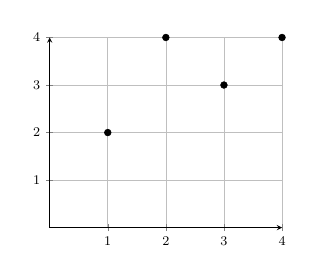
\begin{tikzpicture}[scale=0.6]
    \begin{axis}[
            grid = major,
            xmin=0, xmax=4,
            ymin=0, ymax=4,
            axis lines=center,
            axis on top=true,
            small,
            domain=0:4,
        ]
        \addplot[only marks, color = black, mark = *]
        table[meta=label] {
            x       y       label
            1       2       a
            2       4       a
            3       3       a
            4       4       a
        };
    \end{axis}
    \end{tikzpicture} 
    \caption{polynomial $p$}
\end{figure}

\noindent
Instead of solving the polynomial, we will start to divide the problem into smaller pieces and solve them one by one. We create a polynomial, \begin{math} \lambda_1, \lambda_2, \lambda_3\end{math} and \begin{math}\lambda_4\end{math}, one for each point from polynomial \textit{p}. These polynomial takes value 1 in one point and 0 in the other points. For example \begin{math} \lambda_1\end{math} takes 1 in 1 and 0 in 2,3 and 4.

\begin{figure}[H]
    \centering
    \captionsetup[subfigure]{labelformat=empty}
    \begin{subfigure}[b]{0.3\textwidth}
        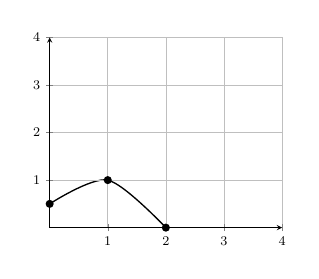
\begin{tikzpicture}[scale=0.6]
        \begin{axis}[
                grid = major,
                xmin=0, xmax=4,
                ymin=0, ymax=4,
                axis lines=center,
                axis on top=true,
                small,
            ]
            \addplot[smooth, thick, color = black, mark = *]
            table[meta=label] {
                x       y       label
                0       0.5     a
                1       1       a
                2       0       a
            };
        \end{axis}
        \end{tikzpicture} 
        \caption{approximately $\lambda_1$}
    \end{subfigure}
    \qquad % <----------------- SPACE BETWEEN PICTURES
    \qquad % <----------------- SPACE BETWEEN PICTURES
    \qquad % <----------------- SPACE BETWEEN PICTURES
    \qquad % <----------------- SPACE BETWEEN PICTURES
    \begin{subfigure}[b]{0.3\textwidth}
        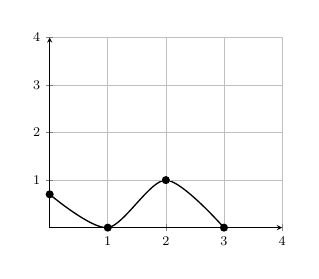
\begin{tikzpicture}[scale=0.6]
        \begin{axis}[
                grid = major,
                xmin=0, xmax=4,
                ymin=0, ymax=4,
                axis lines=center,
                axis on top=true,
                small,
            ]
            \addplot[smooth, thick, color = black, mark = *]
            table[meta=label] {
                x       y       label
                0       0.7     a
                1       0       a
                2       1       a
                3       0       a
            };
        \end{axis}
        \end{tikzpicture} 
        \caption{approximately $\lambda_2$}
    \end{subfigure}
\end{figure}

\noindent
Note that the evaluation in 0 will depend on the secret. For the sake of the drawings it is just an approximately of the point.

\begin{figure}[H]
    \centering
    \captionsetup[subfigure]{labelformat=empty}
    \begin{subfigure}[b]{0.3\textwidth}
        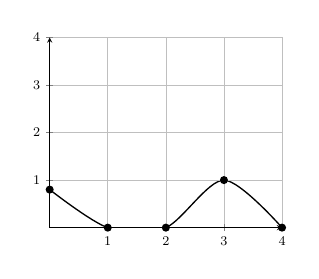
\begin{tikzpicture}[scale=0.6]
        \begin{axis}[
                grid = major,
                xmin=0, xmax=4,
                ymin=0, ymax=4,
                axis lines=center,
                axis on top=true,
                small,
            ]
            \addplot[smooth, thick, color = black, mark = *]
            table[meta=label] {
                x       y       label
                0       0.8     a
                1       0       a
                2       0       a
                3       1       a
                4       0       a
            };
        \end{axis}
        \end{tikzpicture} 
        \caption{approximately $\lambda_3$}
    \end{subfigure}
    \qquad % <----------------- SPACE BETWEEN PICTURES
    \qquad % <----------------- SPACE BETWEEN PICTURES
    \qquad % <----------------- SPACE BETWEEN PICTURES
    \qquad % <----------------- SPACE BETWEEN PICTURES
    \begin{subfigure}[b]{0.3\textwidth}
        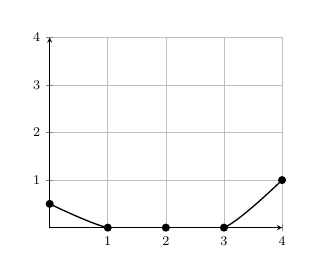
\begin{tikzpicture}[scale=0.6]
        \begin{axis}[
                grid = major,
                xmin=0, xmax=4,
                ymin=0, ymax=4,
                axis lines=center,
                axis on top=true,
                small,
            ]
            \addplot[smooth, thick, color = black, mark = *]
            table[meta=label] {
                x       y       label
                0       0.5     a
                1       0       a
                2       0       a
                3       0       a
                4       1       a
            };           
        \end{axis}
        \end{tikzpicture} 
        \caption{approximately $\lambda_4$}
    \end{subfigure}
\end{figure}

\noindent
To construct the polynomial \begin{math}p\end{math} is to take each polynomials and multiply the corresponding coefficient from \begin{math}p\end{math} and then sum the polynomials together \begin{math}2∙\lambda_1+4∙\lambda_2+3∙\lambda_3+4∙\lambda_4 \end{math}. We started with the polynomial $p$ and we ended with four polynomials, which takes value 2,4,3,4 and 0 in the other points. From the sum we see that the value in the first point 2+0+0+0. It is clear this will work in the other points. 

\begin{figure}[H]
    \centering
    \captionsetup[subfigure]{labelformat=empty}
    \begin{subfigure}[b]{0.3\textwidth}
        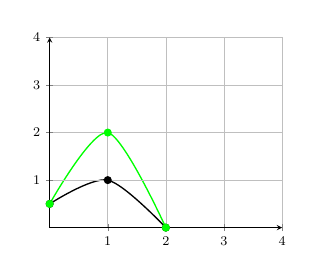
\begin{tikzpicture}[scale=0.6]
        \begin{axis}[
                grid = major,
                xmin=0, xmax=4,
                ymin=0, ymax=4,
                axis lines=center,
                axis on top=true,
                small,
            ]
            \addplot[smooth, thick, color = black, mark = *]
            table[meta=label] {
                x       y       label
                0       0.5     a
                1       1       a
                2       0       a
            };
            \addplot[smooth, thick, color = green, mark = *]
            table[meta=label] {
                x       y       label
                0       0.5     a
                1       2       a
                2       0       a
            };             
        \end{axis}
        \end{tikzpicture} 
        \caption{approximately $\lambda_1$}
    \end{subfigure}
    \qquad % <----------------- SPACE BETWEEN PICTURES
    \qquad % <----------------- SPACE BETWEEN PICTURES
    \qquad % <----------------- SPACE BETWEEN PICTURES
    \qquad % <----------------- SPACE BETWEEN PICTURES
    \begin{subfigure}[b]{0.3\textwidth}
        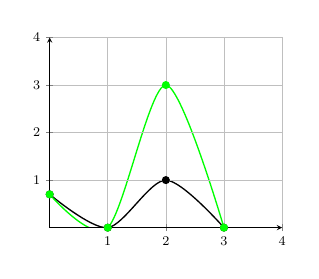
\begin{tikzpicture}[scale=0.6]
        \begin{axis}[
                grid = major,
                xmin=0, xmax=4,
                ymin=0, ymax=4,
                axis lines=center,
                axis on top=true,
                small,
            ]
            \addplot[smooth, thick, color = black, mark = *]
            table[meta=label] {
                x       y       label
                0       0.7     a
                1       0       a
                2       1       a
                3       0       a
            };
            \addplot[smooth, thick, color = green, mark = *]
            table[meta=label] {
                x       y       label
                0       0.7     a
                1       0       a
                2       3       a
                3       0       a
            };             
        \end{axis}
        \end{tikzpicture} 
        \caption{approximately $\lambda_2$}
    \end{subfigure}
\end{figure}

\begin{figure}[H]
    \centering
    \captionsetup[subfigure]{labelformat=empty}
    \begin{subfigure}[b]{0.3\textwidth}
        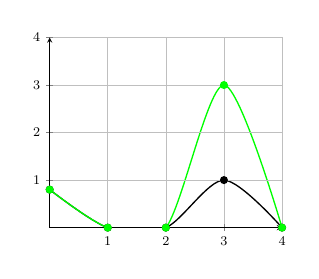
\begin{tikzpicture}[scale=0.6]
        \begin{axis}[
                grid = major,
                xmin=0, xmax=4,
                ymin=0, ymax=4,
                axis lines=center,
                axis on top=true,
                small,
            ]
            \addplot[smooth, thick, color = black, mark = *]
            table[meta=label] {
                x       y       label
                0       0.8     a
                1       0       a
                2       0       a
                3       1       a
                4       0       a
            };
            \addplot[smooth, thick, color = green, mark = *]
            table[meta=label] {
                x       y       label
                0       0.8     a
                1       0       a
                2       0       a
                3       3       a
                4       0       a
            };            
        \end{axis}
        \end{tikzpicture} 
        \caption{approximately $\lambda_3$}
    \end{subfigure}
    \qquad % <----------------- SPACE BETWEEN PICTURES
    \qquad % <----------------- SPACE BETWEEN PICTURES
    \qquad % <----------------- SPACE BETWEEN PICTURES
    \qquad % <----------------- SPACE BETWEEN PICTURES
    \begin{subfigure}[b]{0.3\textwidth}
        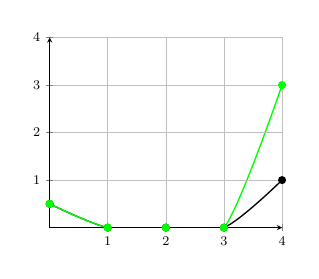
\begin{tikzpicture}[scale=0.6]
        \begin{axis}[
                grid = major,
                xmin=0, xmax=4,
                ymin=0, ymax=4,
                axis lines=center,
                axis on top=true,
                small,
            ]
            \addplot[smooth, thick, color = black, mark = *]
            table[meta=label] {
                x       y       label
                0       0.5     a
                1       0       a
                2       0       a
                3       0       a
                4       1       a
            };
            \addplot[smooth, thick, color = green, mark = *]
            table[meta=label] {
                x       y       label
                0       0.5     a
                1       0       a
                2       0       a
                3       0       a
                4       3       a
            };               
        \end{axis}
        \end{tikzpicture} 
        \caption{approximately $\lambda_4$}
    \end{subfigure}
\end{figure}


\noindent
We will now construct one of the \begin{math}\lambda\end{math}-polynomials by example, by showing it from \begin{math}\lambda_1\end{math} polynomial. 
We have the following points \begin{math}\lambda_1(1)=1, \lambda_1(2)=0, \lambda_1(3)=0 \end{math} and \begin{math} \lambda_1 (4)=0\end{math}. We take the polynomial \begin{math} (x-2)(x-3)(x-4)\end{math}, and we see that if we get correct evaluation in \begin{math}\lambda_1 (2)=0, \lambda_1 (3)=0\end{math} or \begin{math} \lambda_1 (4)=0\end{math}. To get correct evaluation in  \begin{math} \lambda_1 (1)=1\end{math} we divide by \begin{math}-6\end{math} because we see that \begin{math}(1-2)(1-3)(1-4)=-6\end{math} and then we end up with a polynomial \begin{math}\frac{(x-2)(x-3)(x-4)}{(-6)}\end{math} .  The polynomial still satisfies the conditions because when we divide zero with "something" we get zero.  The formula for constructing \begin{math}\lambda_1\end{math} 

\begin{center}
\begin{math} \lambda_1(x)=\prod\limits_{j\in C,j\neq1} \frac{x-j}{1-j} = \frac{x-2}{1-2} \cdot \frac{x-3}{1-3} \cdot \frac{x-4}{1-4}=\frac{(x-2)(x-3)(x-4)}{-6} \end{math}\\
\end{center}

\noindent
\begin{math} \lambda_1\end{math} gives 1 in point 1 and 0 in the other points. What this mean is that in \begin{math} \lambda_1(1)=1\end{math} and all other points  \begin{math}j (2,3,4)\end{math} we have \begin{math} \lambda_1 (j)=0\end{math}. We can construct \begin{math}\lambda_1, \lambda_2, \lambda_3\end{math} and  \begin{math}\lambda_4\end{math} in the same way.

\begin{center}
\begin{math} \lambda_2(x)=\prod\limits_{j\in C,j\neq2} \frac{x-j}{2-j} = \frac{x-1}{2-1} \cdot \frac{x-3}{2-3} \cdot \frac{x-4}{2-4}=\frac{(x-1)(x-3)(x-4)}{-2} \end{math}\\ 

\begin{math} \lambda_3(x)=\prod\limits_{j\in C,j\neq3} \frac{x-j}{3-j} = \frac{x-1}{3-1} \cdot \frac{x-3}{3-2} \cdot \frac{x-4}{3-4}=\frac{(x-1)(x-2)(x-4)}{-2} \end{math}\\ 

\begin{math} \lambda_4(x)=\prod\limits_{j\in C,j\neq4} \frac{x-j}{4-j} = \frac{x-1}{4-1} \cdot \frac{x-3}{4-2} \cdot \frac{x-3}{4-3}=\frac{(x-1)(x-2)(x-3)}{-6} \end{math}\\ 
\end{center}

\noindent
With the knowledge of the evaluation of \begin{math}p(1), p(2), p(3)\end{math} and  \begin{math}p(4)\end{math} we construct the formula for polynomial evaluation in \begin{math}p(0)\end{math}. We use the Lagrange polynomial interpolation formula \begin{math}p(x)=\sum\limits_{i \in C} p(i)\lambda_i(x)\end{math} and we get the evaluation on some polynomial in $0$.


\noindent
\begin{alignat*}{4}
p(0) &=p(1)∙\lambda_1+p(2)∙\lambda_2+p(3)∙\lambda_3+p(4)∙\lambda_4=2∙\lambda_1+4∙\lambda_2+3∙\lambda_3+4∙\lambda_4  
\end{alignat*}



\noindent
The idea of constructing the smaller polynomials is that we can reuse them for constructing other polynomials. From the smaller pieces and the evaluation points we can construct the polynomial from Lagrange interpolation. From the secret sharing scheme we know the degree of the polynomial is bounded. Because the voter will share its secret by choosing a random polynomial of the degree at most \textit{t-1}.Then we need $t$ point to reconstruct the $p(x)$. If the degree 1 (line) then we need two points. The parable is where the degree is 2, here we need 3 points to construct
the polynomial etc.

\begin{figure}[H]
    \centering
    \captionsetup[subfigure]{labelformat=empty}
    \begin{subfigure}[b]{0.3\textwidth}
        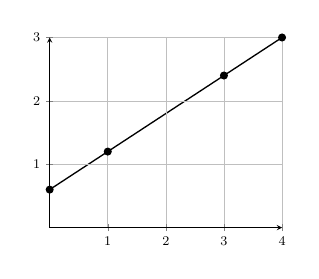
\begin{tikzpicture}[scale=0.6]
        \begin{axis}[
                grid = major,
                xmin=0, xmax=4,
                ymin=0, ymax=3,
                axis lines=center,
                axis on top=true,
                small,
            ]
            \addplot[smooth, thick, color = black, mark = *]
            table[meta=label] {
                x       y       label
                0       0.6     a
                1       1.2     a
                3       2.4     a
                4       3       a
            };
        \end{axis}
        \end{tikzpicture} 
        \caption{polynomial of degree 1}
    \end{subfigure}
    \qquad % <----------------- SPACE BETWEEN PICTURES
    \qquad % <----------------- SPACE BETWEEN PICTURES
    \qquad % <----------------- SPACE BETWEEN PICTURES
    \qquad % <----------------- SPACE BETWEEN PICTURES
    \begin{subfigure}[b]{0.3\textwidth}
        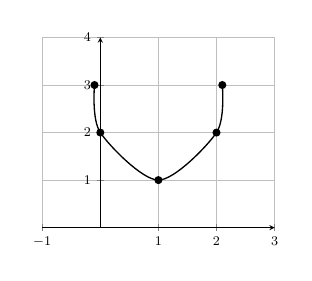
\begin{tikzpicture}[scale=0.6]
        \begin{axis}[
                grid = major,
                xmin=-1, xmax=3,
                ymin=0, ymax=4,
                axis lines=center,
                axis on top=true,
                small,
            ]
            \addplot[smooth, thick, color = black, mark = *]
            table[meta=label] {
                x       y       label
                -0.1    3       a
                0       2       a
                1       1       a
                2       2       a
                2.1     3

            };           
        \end{axis}
        \end{tikzpicture} 
        \caption{polynomial of degree 2}
    \end{subfigure}
\end{figure}


\parahead{In the PVSS protocol} we will use a simplified version of Lagrange interpolation formula. So instead of recovering the polynomium we just recover the evaluation in zero. The following will happen if take the formula \begin{math} \lambda_i(x)=\prod\limits_{j\in C,j\neq i}  \frac{x-j}{i-j} \end{math} and evaluate in zero \begin{math} \lambda_i(0)=\prod\limits_{j\in C,j\neq i}  \frac{0-j}{i-j} = \prod\limits_{j\in C,j\neq i} \frac{j}{j-i} \end{math}. We reduce the formula by evaluating in $0$ and then one can multiply the numerator and denominator by $-1$ and then we get a the above formula. Below we computed the coefficients for 3 static participants. These coefficients will be used in our simplified example of the protocol in appendex \ref{sec:simple_review_of_calculations_in_the_protocol}.


\noindent
\begin{alignat*}{4}
\lambda_1(0) &=\prod\limits_{j\in C,j\neq 1} \frac{2}{2-1}  \cdot  \frac{3}{3-1} &&=\frac{3}{1} = 3 \\
\lambda_2(0) &=\prod\limits_{j\in C,j\neq 2} \frac{1}{1-2}  \cdot  \frac{3}{3-2} &&=\frac{1}{-1} \cdot  \frac{3}{1} =-1 \cdot  3=-3 \\
\lambda_3(0) &=\prod\limits_{j\in C,j\neq 3} \frac{1}{1-3}  \cdot  \frac{2}{2-3} &&=\frac{1}{-2} \cdot  \frac{2}{-1} =1  
\end{alignat*}




 \subsection{Example computation using Shamir Secret Sharing}
  \label{sec:example_computation_using_shamir_secret_sharing}
We have now explained the basic for secret sharing. This section will show a full concrete computational example on distribution and reconstruction of a secret between 5 participant where we want to tolerate $t=2$ corrupted parties. The computation is computed in $\Z_{11}^*$. The example is that one participant, $p_1$, has a secret, $s=7$ and creates shares to the other participants ($p_2, p_3, p_4, p_5$). Then if $3$ participants combines the shares they will be able to reconstruct the secret. \\

\noindent
First the participant $p_1$ creates a random polynomium, $p(x)$ at degree $t=2$ which is the following polynomium $p(x)=s + a_{1}x+ a_{2}x^2$, where $s=7$ is the secret and $a_{1}=4$ and $a_{2}=1$ is coefficient uniformly randomly choosen from $\Z_{11}$. The following will show the distribution where $p_1$ create shares to the other parties. In the reconstruction we show how $3$ parties will be able to reconstruct the polynomial and the secret by their shares using Lagrange interpolation.   

\subsubsection{Distribution}
The shares $s_1, s_2, s_3, s_4,s_5$ is computed from $p(x)=7 + 4x+ x^2$ as

\noindent
\begin{alignat*}{4}
s&=p(0)&&= 7+0+0 \ &&(mod \ 11) &&=7 \\
s_1&=p(1)&&= 7+4+1 \ &&(mod \ 11) &&=1 \\
s_2&=p(2)&&= 7+8+4 \ &&(mod \ 11) &&=8 \\
s_3&=p(3)&&= 7+12+9 \ &&(mod \ 11) &&=6 \\
s_4&=p(4)&&= 7+16+16 \ &&(mod \ 11) &&=6 \\
s_5&=p(5)&&= 7+20+25 \ &&(mod \ 11) &&=8    
\end{alignat*}


\noindent
Each party now recieve their shares secure. So $p_2= s_2, p_3=s_3, p_4= s_4, p_5= s_5$. No that the secret is $p(0)=s= 7$.

\subsubsection{Reconstruction}
A subset, $3>2$, of participant $p_3, p_4, p_5$ wants to reconstruct the secret by their shares using Lagrange interpolation. First every party computes a polynomial. After that the parties will be able to combine their polynomial and their shares to reconstruct $p(x)$.\\

%------------------------------------------------------------------------------------
\noindent
$p_3$ computes:
%------------------------------------------------------------------------------------


\noindent
\begin{alignat*}{3}
\lambda_3(x)&=\prod\limits_{j\in C,j\neq3} \frac{x-j}{3-j} = \frac{x-4}{3-4} \cdot \frac{x-5}{3-5} =\frac{(x-4)(x-5)}{(3-4)(3-5)}  \\
&= (x^2-9x+20)((3-4)(3-5))^{-1} \ (mod \ 11)
\end{alignat*}

\noindent
The inverse of  $((3-4)(3-5))= 2$ is $6$ since $2 \cdot 6 \ mod \ 11 = 1$. We now have the following polynomial

\noindent
\begin{alignat*}{3}
\lambda_3(x) = (x^2-9x+20)6 \ (mod \ 11) &= (x^2 + 2x+9)6 \ &(mod \ 11) \\
&= 6x^2 + 12x + 54 \ &(mod \ 11) \\
&= 6x^2+x+ 10 \ &(mod \ 11) 
\end{alignat*}

\noindent
We verify the following


\noindent
\begin{alignat*}{6}
\lambda_3(3) &=  6 \cdot 3^2+3+ 10  \ &&(mod \ 11) &&= 67 \ &&(mod \ 11) &&= 1 \\
\lambda_3(4) &=  6 \cdot 4^2+4+ 10  \ &&(mod \ 11) &&= 110 \ &&(mod \ 11) &&= 0 \\
\lambda_3(5) &=  6 \cdot 5^2+5+ 10  \ &&(mod \ 11) &&= 165 \ &&(mod \ 11) &&= 0
\end{alignat*}

%------------------------------------------------------------------------------------
\noindent
$p_4$ computes:
%------------------------------------------------------------------------------------

\noindent
\begin{alignat*}{3}
 \lambda_4(x)&=\prod\limits_{j\in C,j\neq4} \frac{x-j}{4-j} = \frac{x-3}{4-3} \cdot \frac{x-5}{4-5} =\frac{(x-3)(x-5)}{(4-3)(4-5)}\\ 
 &= (x^2-8x+15)((4-3)(4-5))^{-1} \ (mod \ 11)
\end{alignat*}



\noindent
The inverse of  $((4-3)(4-5))= -1$ is $10$ since $-1 \cdot 10 \ (mod \ 11) = 1$. We now have the following polynomial


\noindent
\begin{alignat*}{3}
\lambda_4(x) = (x^2-8x+15)10 \ (mod \ 11) &= (x^2 + 3x+4)10 \ &&(mod \ 11) \\
                                          &= 10x^2 + 8x + 7 \ &&(mod \ 11) 
\end{alignat*}

\noindent
We verify the following

\noindent
\begin{alignat*}{3}
\lambda_4(3) &=  10 \cdot 3^2+24+ 7  \ (mod \ 11) &&= 121 \ (mod \ 11) = 0 \\
\lambda_4(4) &=  10 \cdot 4^2+32+ 7  \ (mod \ 11) &&= 199 \ (mod \ 11) = 1 \\
\lambda_4(5) &=  10 \cdot 5^2+40+ 7  \ (mod \ 11) &&= 297 \ (mod \ 11) = 0 \\
\end{alignat*}




%------------------------------------------------------------------------------------
\noindent
$p_5$ computes:
%------------------------------------------------------------------------------------

\noindent
\begin{alignat*}{3}
 \lambda_5(x)&=\prod\limits_{j\in C,j\neq5} \frac{x-j}{5-j} = \frac{x-3}{5-3} \cdot \frac{x-4}{5-4} =\frac{(x-3)(x-4)}{(5-3)(5-4)} \\
&= (x^2-7x+12)((5-3)(5-4))^{-1} \ (mod \ 11)
\end{alignat*}



\noindent
The inverse of  $((5-3)(5-4))= 2$ is $6$ since $2 \cdot 6 \ mod \ 11 = 1$. We now have the following polynomial

\noindent
\begin{alignat*}{3}
\lambda_5(x)= (x^2-7x+12)6 \ (mod \ 11) &= (x^2 + 4x+1)6 \ &&(mod \ 11) \\
                                        &= 6x^2 + 24x + 6 \ &&(mod \ 11) \\
                                        &= 6x^2 + 2x + 6 \ &&(mod \ 11)
\end{alignat*}

\noindent
We verify the following

\noindent
\begin{alignat*}{6}
\lambda_5(3) &=  6 \cdot 3^2+6+ 6  \ &&(mod \ 11) &&= 66 \ &&(mod \ 11)  &&= 0 \\
\lambda_5(4) &=  6 \cdot 4^2+8+ 6  \ &&(mod \ 11) &&= 110 \ &&(mod \ 11) &&= 0 \\
\lambda_5(5) &=  6 \cdot 5^2+10+6  \ &&(mod \ 11) &&= 166 \ &&(mod \ 11) &&= 1  
\end{alignat*}




\noindent
To construct the polynomial \begin{math}p\end{math} we take each polynomials and multiply by the corresponding shares. More formally we apply \begin{math}p(x)=\sum\limits_{i \in C} p(i)\lambda_i(x)\end{math} to construct the $p(x)$.



\noindent
 \begin{alignat*}{2}
p(x) &= s_3 \lambda_3 (x) + s_4 \lambda_4 (x) + s_5 \lambda_5 (x) &\\
     &= s_3(6x^2+x+ 10) + s_4(10x^2 + 8x + 7)  + s_5(6x^2 + 2x + 6)&\\
     &= (6s_3+10s_4+6s_5)x^2 + (s_3 + 8s_4 + 2s_5)x  + (10s_3 + 7s_4 + 6s_5)&
\end{alignat*} 
   

\noindent
Since the polynomial is of the form $p(x)=s + a_{1}x+ a_{2}x^2$ we have that

\noindent
\begin{alignat*}{2}
s&  = 10s_3 + 7s_4 + 6s_5 \ &&(mod \ 11)  \\
a_1&= s_3 + 8s_4 + 2s_5\ &&(mod \ 11) \\
a_2&= 6s_3+10s_4+6s_5\ &&(mod \ 11) 
\end{alignat*} 

\noindent
We can now replace the variables with shares $s_3=6, s_4=6, s_5=8$

\noindent
\begin{alignat*}{6}
s&  = 10 \cdot 6 + 7 \cdot 6 + 6 \cdot 8 \ &&(mod \ 11)  &&= 150  \ &&(mod \ 11) &&= 7\\
a_1&= 6 + 8 \cdot 6 + 2 \cdot 8 \ &&(mod \ 11) &&= 70  \ &&(mod \ 11) &&= 4\\
a_2&= 6 \cdot 6 +10 \cdot 6+ 6 \cdot 8 \ &&(mod \ 11) &&= 144  \ &&(mod \ 11) &&= 1
\end{alignat*}

\noindent
The reconstruction gives us the final polynomial $p(x)=7 + 4x+ x^2$ and thereby the secret value $7$.


\subsection{Verifiable Secret Sharing (VSS)}
Where the basic model of secret sharing assumes that every participants involved is honest, the VSS requires its participants to prove so. The objective of the VSS is to resist malicious participants such as malicious participants can mislead as follows \cite{Schoenmakers1999}

\begin{itemize}
    \item Dealer is sending incorrect shares to some or all participants in the distribution phase
    \item Participants is submitting incorrect shares during the reconstruction phase
\end{itemize}

\noindent 
By requiring proof of correctness of the shares, from the participants, in the distribution and the reconstruction phase, the VSS model solves the problem of malicious participants. These proofs is constructed in such a way that only the participants is able to construct and verify the proofs. Where it is a logical requirement that only the participants is able to construct the proofs, it is a different story with the verification. In fact in most case it would be ideal if anybody could validate the proofs. 


\subsection{Public Verifiable Secret Sharing (PVSS)}
In a PVSS schemes it is required that, not only the participants but anybody, is able to validate the shares. It is therefore not assumed that there are private channels between the participants. All communication in PVSS schemes  is done over authenticated public channels using public key encryption, which also means that the secret is only computationally hidden. A common structure for the PVSS protocols is as follows.

\begin{description}
    \item[Initialization] Each participants registers itself and must have a public key.  
    
    \item[Distribution] consists of a distribution and a verification phase
    
    \begin{enumerate}
        \item \textit{Distribution of the shares}
        \begin{enumerate}
            \item \textit{Dealer creates shares}
            \item \textit{Dealer publishes encrypted shares}    
            \item \textit{Dealer publishes a $proof_D$}   
        \end{enumerate}
        \item \textit{Verification of the shares} 
        \begin{enumerate}
            \item \textit{Anybody who knows the public key can verifier the shares}
            \item \textit{If the verification on $proof_D$ fails the dealer fails and the protocol is aborted}  
        \end{enumerate}
    \end{enumerate}
    
    
    \item[Reconstruction] consists of a decryption phase and pooling the shares phase    
        
    \begin{enumerate}
        \item \textit{Decryption of the shares}
         \begin{enumerate}
            \item \textit{The participants decrypt their shares}
            \item \textit{The participants publishes a $proof_{p_{i}}$}  
        \end{enumerate}
        \item \textit{Pooling the shares}  
        \begin{enumerate}
            \item \textit{$proof_{p_{i}}$ are used to exclude dishonest participants}
            \item \textit{Reconstruction of the secret by any qualified set of participants}  
        \end{enumerate}
    \end{enumerate}        

\end{description}

%------------------------------------------------------------------------------------
\subsection{Homomorphic Secret Sharing}
%------------------------------------------------------------------------------------
A homomorphism is a transformation from one algebraic structure into another of the same type so that the structure is preserved. Importantly, this means that for every kind of manipulation of the original data, there is a corresponding manipulation of the transformed data.\\

\noindent 
A homomorphic encryption scheme is a crypto system that allows computations to be performed on data without decrypting it. It is an encrypting scheme which allows computations to be carried out on ciphertext, thus generating an encrypted result which, when decrypted, matches the result of operations performed on the plaintext.\\

\noindent 
Homomorphic Secret Sharing is a type of secret sharing algorithm in which the secret is encrypted via homomorphic encryption. In the PVSS scheme we use this property that one can sum the shares which are equal to the sum of the secrets.


    
    
 \clearpage
%***************************************************************
%               Part 5: The Protocol
%***************************************************************  
\chapter{Electronic voting protocol}
    In this section we look at the electronic voting protocol described in \cite{Schoenmakers1999}. The protocol is based on the PVSS protocol described in the same article. We will only describe the electronic voting protocol but as doing so, the relevant elements from the PVSS protocol will be taking into the description. For the rest of this chapter we will be referring to the electronic voting protocol, as simply the protocol, unless specified otherwise. \\

\noindent
Giving the complexity of the protocol we divided this description into three parts. In the first part we will describe the protocol as simple as possible, leaving out mathematical justification and proofs.  We provide a calculated example for low values for the basic parts of the protocol in \ref{sec:simple_review_of_calculations_in_the_protocol}.  In second part we will be looking at the mathematical justification, describing this in the same order as in the first part. Finally we will look at the proofs in the last part. 


%--------------------------------------------------------------------------
\section{The protocol}   \label{sec:the_protocol}
%--------------------------------------------------------------------------


\noindent
The overall concept of the protocol is to allow a group of voters to cast there votes in the form "no" or "yes" , and publish the result to a public bulletin board. When a deadline is reach or when all votes have been casted a group of talliers takes the votes and calculates the end result. 
Using MPC and PVSS protocols this is done in such a way that none other then the voter knows the value of his vote, but everyone can validates the correctness and consistence of the vote. Below we present a simple overview showing the progress of the protocol. \\

\noindent
\textbf{Short overview of the protocol}
The protocol is divided into three main parts, each part representing a different phase in the election, roughly put one can say pre-election, the election and post-election. 

\noindent
\begin{enumerate}
    \item \textbf{Initialization}
    This represents the pre-election phase where the preparation for the actually election happens. Here the requirements for the election is demented and the different authorities is registered. 
    
        \begin{enumerate}
            \item The system publishes the system parameters and the security requirements. In our implementation an admin user will log into the system and start the election. The admin will choose the security parameter and the amount of required talliers. Last he will initiate the computation of the system parameters.
            
            \item Each tallier generates a private and a public key.
            
            \item Each tallier registries their public keys on the bulletin board.
            
            \item Each voter signs it credentials on the bulletin board.
        \end{enumerate}
        
    \item \textbf{Ballot casting}
    This represent the actually election, where the registered voters castes there votes and publish the result to the bulletin board. 
    
        \begin{enumerate}
            \item Each voter votes $1$ or $0$
        
            \item Each voter generates a random secret.
        
            \item Each voter creates shares of the secret to each tallier and encrypts it with the corresponding public key of the tallier. Each voter supply this secret share with evidence of its consistency with a $DLEQ$ proof.
        
            \item Each voter supply evidence for a valid vote with $PROOF_U$.
        \end{enumerate}
        
    \item \textbf{Tallying} 
    This represents the post-election phase where the tallying authorities, which where registered in Initialization, counts the votes together and publish the result to the bulletin board.
    
        \begin{enumerate}
            \item At least $t$ tallier accumulates and decrypts their shares.
            
            \item One authority completes the final computation of the total votes.
        \end{enumerate}
\end{enumerate}


\noindent
In the following we will describe the central parts of the protocol, leaving out the complexity of mathematical justification and proofs. The idea is to get an understanding of how the protocol works without know exactly why it works. \\

\noindent
For efficiency we will limit the computation of the votes to a finite number of talliers. There are \textit{m} voters and \textit{n} talliers.
%--------------------------------------------------------------------------
\subsection{Initialization}   \label{sec:the_protocol_initialization}
%--------------------------------------------------------------------------

\noindent
\textbf{The bulletin board publishes all system parameters which is the public elements a prime $q$,  the generators $g$ and $G$ and a security parameter $t$.}


\begin{alignat*}{2}
q \ &\in_R \{2^{l-1},...,2^{l}\}, \ where\  l &&> 1024 \\
f \ &\in_R \{2,...,2q-1\} \rightarrow g &&= f^2 \ mod\ 2q+1  \\
F \ &\in_R \{2,...,2q-1\}\rightarrow G &&= F^2 \ mod\ 2q+1 \\
t &\in \Z_q^* &&= \{1,2,3,...,q-1\} 
\end{alignat*}

\noindent
The prime $q$ is uniformly randomly chosen from $\Z$, but in practise we use the subset $2^{l-1}$ to $2^l$. $l$ is chosen  larger then 1024 because of the security requirements described in section \ref{sec:solving_the_discrete_logarithm_problem}. The generators $g$ and $G$ are computed as squares from the sets $f$ and $F$, the reason for this is elaborated in section \ref{sec:protocol_details_initialization}.  $2q+1$ must also be a prime and the reason why we use $2q +1$ is because we are working with Shamirs secret sharing in the exponents which also is described in section \ref{sec:protocol_details_initialization}. $t$ is chosen based on the system requirements for our fault tolerance against corrupted parties.\\

\noindent
\textbf{The tallier generates a private key $x_i$ and a public key $y_i$.}
\begin{flalign*}
Private \ key &: x_{i} \in_R \Z_q^* = \{1,2,3,...,q-1\}\\
Public \ key &: y_i=G^{x_i} ,\ i \in \{1,2,3,...., n \}
\end{flalign*}

\noindent
Every tally generates a uniformly randomly chosen private key from $\Z_q^*$ where $q$ is a prime. The star notation refers to a set with none greatest common divisor larger then $1$ respectively with $q$, which is described in section \ref{sec:group_theory}. The public key is computed on an exponentation on $G$, which essentially gives us the security of the discrete logarithm problem described in section ~\ref{sec:discrete_logarithm_problem}.

%--------------------------------------------------------------------------
\subsection{Ballot casting}
\label{sec:ballot_casting}
%--------------------------------------------------------------------------
The  Ballot casting consists of \textit{distribution of the shares} and \textit{verification of the shares}.\\

\noindent
First the voter either votes "no" or "yes" corresponding to 0 or 1. The voter select a uniformly random secret $s \in \Z_q$. The PVSS protocol is then used to distribute shares which contain a combination of the secret $s$ and the vote. Every voter will construct a random polynomial at degree $t-1$ and then evaluate the shares  to each of the talliers.\\


\noindent
\textbf{The voter casts his vote, either 0 or 1. The voter creates a random secret $s$ and a random polynomial of degree at most $t-1$ and computes the shares.}

\begin{flalign*}
Vote &: v\in\{0,1\} & \\
Random \ secret  &: s\in_R \Z_q &\\
Random \ polynomium &:  p(x)=s+\alpha_1x^1+\alpha_2x^2+,...,+\alpha_{t-1}x^{t-1}, \ \alpha_j\in_R \Z_q &\\
Secret \ Shares &:  p(0)=s,\ p(1),\ p(2),...,\ p(n)
\end{flalign*}

\noindent
The degree of the polynomium is based on the security parameter $t$ described in section ~\ref{sec:the_protocol_initialization}. Each voter chooses uniformly random the coefficients $\alpha$ in $Z_q$ and a random secret $s$ and computes the shares using Shamirs secret sharing which is described in section \ref{sec:example_computation_using_shamir_secret_sharing}.\\

\noindent
\textbf{The voter distributes the encrypted share and creates the proofs $PROOF_U$ and $DLEQ$.}

\begin{alignat*}{2}
Encryption \ of \ the \ share : Y_i&=y_i^{p(i)} ,1\leq i\leq n \\ 
Hidden \ vote : U&=G^{s+v}
\end{alignat*}

\noindent
Each voter creates encrypted shares to tally $1$, tally $2$,..., tally $n$. The $p(i)$ refers to the share in a point corresponding to a given tally. The shares are encrypted using the tallys public key $y_i$. $U$ is a DL problem that hides the vote as the exponentiation. As the vote $v$ only can hold the values $0$ or $1$ this wouldn't make a hard problem. By reusing the secret $s$ and adding this to $v$, then given a large $s$, $U$ should be a hard problem. The above is then published to the bulletin board. \\

\noindent
Besides the above, the proofs $PROOF_U$ and $DLEQ$ are computed and published. The $PROOF_U$ proofs that the vote is either $0$ or $1$ without revealing the actual value of the vote. The $DLEQ$ proofs that the shares are constructed correctly and consistent. Both proofs are elaborated in details later in section \ref{sec:proofs}

%--------------------------------------------------------------------------
\subsection{Tallying}
\label{sec:tallying}
%--------------------------------------------------------------------------
Tallying is the process of counting the votes. Here the tallier uses their private keys to collectively compute the final tally, based on the valid ballots.\\



\noindent
\textbf{The tally decrypts their shares and publishes a $DLEQ$ proof}

\begin{flalign*}
Multiplum \ of \ encrypted \ shares &: Y_i^*=(\prod\limits_{j=1}^{m} Y_{ij}) \ (mod\ 2 \cdot q+1)
\end{flalign*}

\noindent
The homomorphic secret sharing property ensures that each tally will  be able to multiply the shares and then decrypt. Let $Y_{ij}$ be the value $Y_i$ computed by the $j$-th voter, which is the encrypted share $Y_i = y_i^{p(i)}$,  as described in the section \ref{sec:ballot_casting}. This means that the $i$ is referring to tally 1, tally  2 and tally 3 etc. and $j$ is referring to voter 1, voter 2 and voter 3 etc. $Y_i^*$ is then the multiplum of encrypted shares for a given tally $i$. Tally $i$ is now able to decrypt the multiplum $Y_i^*$ using his private key $x_i$. 

\begin{flalign*}
Decrypted \ multiplum \ of \ shares &: S_i^*=(Y_{i}^*)^{\frac{1}{x_i}} \ (mod\ 2 \cdot q+1)
\end{flalign*}

\noindent
$S_i^*$ is the decrypted multiplum of all tally $i$ shares. As this is the multiplum of shares then no information of the individual share is revealed and tally $i$ can safely publish the decrypted result to the bulletin board.

\noindent
Note that besides decrypting the shares the talliers will publish a $DLEQ$ proof which shows that the decrypting was done correct. See figure \ref{fig:DLEQ_by_talliers} of the $DLEQ$ proof. Also note that we need to computing the inverse of the key $x_i$. To compute the inverse we can use Extended Euclidean algorithm described in section \ref{sec:modular_arithmetic}.\\


\noindent
\textbf{A master authority applies Lagrange interpolation}\\
After the tallier has published their decrypted shares $S_i^*$ a master authority will be able to compute the sum of the secrets from the voters.


\begin{alignat*}{2}
(S_1^*)^{\lambda_1  \cdot  \ (mod \ q)}  \cdot  (S_2^*)^{\lambda_2 \ (mod \ q)}  \cdot  (S_n^*)^{\lambda_n \ (mod \ q)} \ (mod \ 2 \cdot q+1) = G^{ \sum\limits_{j=1}^m s_j}
\end{alignat*}

\noindent
With all the $S_i^*$ we can compute the sum of the secrets. We apply the lambdas to exponents on $S_i^*$, which is computed from the  Lagrange interpolation formular, \begin{math} \lambda_j \end{math} from section \ref{sec:shamir_secret_sharing_lagrange_interpolation}. We can then multiply the $S_i^*$ which can be  reduces to the sum of the exponents, which are equal to the sum of the secrets.\\


\noindent
\textbf{A master authority computes the votes}\\
The last step is to isolate the votes and then compute the final result. By multiplying \begin{math}U_j \end{math} from the voters we obtain the following.

\begin{alignat*}{2}
(\prod\limits_{j=1}^{m} U_{j}) \ (mod \ 2 \cdot q+1)=  G^{ \sum\limits_{j=1}^m s_j +v_j}
\end{alignat*}

\noindent
From the previous step we computed $G^{ \sum\limits_{j=1}^m s_j}$. To  isolate the sum of votes \textit{v} in the exponent we can multiply  $(\prod\limits_{j=1}^{m} U_{j})$ by the inverse of $(G^{ \sum\limits_{j=1}^m s_j})^{-1}$ in the following.

\begin{alignat*}{2}
 G^{ \sum\limits_{j=1}^m s_j +v_j} \cdot (G^{ \sum\limits_{j=1}^m s_j})^{-1} = G^{ \sum\limits_{j=1}^m v_j}
\end{alignat*}


\noindent
To solve the computing of the votes one can compute \begin{math}G^0, G^1, G^3,..., G^{v_j} \end{math} by exhaustive search. The final vote count will be the exponent raised on $G$. A more efficient algorithm is to use Baby-step giant-step algorithm described in section \ref{sec:solving_the_discrete_logarithm_problem}. 

%--------------------------------------------------------------------------
\section{Protocol details} \label{sec:protocol_details}
%--------------------------------------------------------------------------
In this part we will elaborate on the mathematical justification based on our explanation of the protocol.  


\subsection{Initialization} \label{sec:protocol_details_initialization}
\textbf{Elaboration of computation of  $2q+1$}\\
In our implementation we will pick a prime, \begin{math}q\end{math}, so we avoid doing the gcd computation. The protocol states that we have to compute in a group of order $q$. This means that when we are doing operations in the exponent this property should be satisfied \begin{math}g^q=1\end{math} where \begin{math}q\end{math} is prime. If we are doing \begin{math}mod \ q \end{math} in the exponent we have \begin{math}g^q=g^0\end{math}. The reason for doing operation in the exponent \begin{math}mod \ q\end{math} is because we are using Sharmir secret sharing which require a finite field.\\

\noindent
One can see that given a generator $g=2 $ and a prime $q=5$, then \begin{math}2^5 \ mod \ 5 = 32 \ mod \ 5 = 2\end{math}. For this to be true, we take the square of numbers modulo a prime in this form \begin{math}2q+1\end{math}. This is also called a strong prime. By using this mathematical structure this property holds. We can choose \begin{math}b=a^2\end{math}. Then we see the property holds \begin{math}b^{q} = 1 \ mod \ 2q+1\end{math}. Using the same values as before, it is clear that \begin{math}(2^2)^5 \ mod \ 11 = 1024 \ mod \ 11 = 1\end{math}. Fermat little theorem states that \begin{math}b^{q-1} \ mod \ q = 1\end{math} where \begin{math}q\end{math} is prime. So we know if we pick our \begin{math}q\end{math} and \begin{math}b\end{math} (as a square)  in this form \begin{math}(a^{2})^{q+1-1} \ mod \ 2q+1 =1 =  a^{2q} \ mod \ 2q+1 =1\end{math} the property holds. This means if we are working in the exponents we $(mod \ q)$ and if we are working in the bases we $(mod \ 2q+1)$.\\

\noindent
\textbf{Elaboration of the generators}\\
The generators is randomly chosen in the set between $2$ and $2q-1$.  We remove $1$ because if $1$ get squared it will always gives $1$ and can therefor not be used as a generator. We remove $2q$ because $(2q)^2 = 1 \ mod \ 2q+1$. That means if you square $2q$ it will also give $1$ and can therefor not be used as a generator.

\subsection{Ballot casting}

\textbf{Elaboration of computation of  $Y_i$}\\
The $Y_i$ is the shares encrypted using the talliers public key $y_i$ as described in section \ref{sec:ballot_casting}.
 
\begin{alignat*}{5}
&Voter \ 1 &&: Y_{1,1}&&=y_{1,1}^{p_1(1)},Y_{2,1}&&=y_{2,1}^{p_2(2)} ,.., Y_{n,1}&&=y_n^{p_n(n)}\\
&Voter \ 2 &&: Y_{1,2}&&=y_{1,2}^{p_1(1)},Y_{2,2}&&=y_{2,2}^{p_2(2)} ,.., Y_{n,2}&&=y_n^{p_n(n)}\\
&Voter \ \textit{m}&&: Y_{1,m}&&=y_{1,m}^{p_1(1)} , Y_{2,m}&&=y_{2,m}^{p_2(2)} ,.., Y_{n,m}&&=y_n^{p_n(n)}
\end{alignat*}


\noindent
When computing the encryption of the shares $Y_i$, then each voter will compute the above to each of the talliers. For clarification we add the tally to the notation such that we have $Y_{ij}$ where $i$ is the $i$-th tally and $j$ is the $j$-th voter referring to $ Y_{1,1}, \  Y_{1,2}$ etc. \\


\noindent
\textbf{Constructing the variable $C_j$ and $X_i$ to proofs  $DLEQ$ and $Proofu$}\\
As briefly described in section \ref{sec:ballot_casting}, the voter publishes proofs that he have voted and distributed this vote accurately. The proof $Proofu$ uses the variable $C_0$ and the $DLEQ$ uses the variable $X_i$. In order to construct the proofs each voter creates the following variables. 

\begin{flalign*}
&hidden \ coeffiens : C_j = g^{\alpha_j},\ j \in \{0,1,2,3,....,t-1 \}, \ where \ \alpha_0 = s  \\ 
&multiplum \ of \ hidden \ coeffiens: X_i = \prod\limits_{j=0}^{t-1} C_j^{i^j} =g^{p(i)}, \ 1\leq i\leq n \\ 
\end{flalign*}

\noindent
$C_j$ holds all the coeffiens $\alpha_j$ including the secret $\alpha_0$, as these are hidden in the exponent of $g$, this is secured by the DL problem.\\

\noindent
The $p(i)$ raised in the exponent of $g$ is the polynomial $p(i)=\alpha_0+\alpha_1i^1+\alpha_2i^2+,...,+\alpha_{t-1}i^{t-1}$ created by each voter in the Ballot casting phase described in section ~\ref{sec:ballot_casting}.  The way we can reduce the following statement  $X_i = \prod\limits_{j=0}^{t-1} C_j^{i^j}$ to $g^{p(i)}$ is as follows. 

\begin{flalign*}
 X_i = \prod\limits_{j=0}^{t-1} C_j^{i^j} = \prod\limits_{j=0}^{t-1} (g^{\alpha_j})^{i^j} =g^{ \sum\limits_{j=0}^{t-1} \alpha_j \cdot i^{j}} = g^{ \alpha_0 \cdot i^{0} + \alpha_1 \cdot i^{1}+ \alpha_2 \cdot i^{2},..., \alpha_{t-1} \cdot i^{t-1} }  = g^{p(i)}
\end{flalign*}


\noindent
To clarify, if the voter creates $3$ shares, that means the voter has to compute $X_1$, $X_2$ and $X_3$  which means one $X_i$ foreach share. This makes sense because the voter has to prove his honesty foreach of the shares.


\begin{alignat*}{3}
X_1 &=\prod\limits_{j=0}^{t-1} C_j^{i^j} &&= C_0^{1^0}  \cdot  C_1^{1^1}  \cdot  C_2^{1^2} &&=  g^{ \alpha_0 \cdot 1^{0} + \alpha_1 \cdot 1^{1}+ \alpha_2 \cdot 1^{2}}  = g^{p(1)}\\
X_2 &=\prod\limits_{j=0}^{t-1} C_j^{i^j} &&= C_0^{2^0}  \cdot  C_1^{2^1}  \cdot  C_2^{2^2}  &&=  g^{ \alpha_0 \cdot 2^{0} + \alpha_1 \cdot 2^{1}+ \alpha_2 \cdot 2^{2}}  = g^{p(2)}\\
X_3 &=\prod\limits_{j=0}^{t-1} C_j^{i^j} &&= C_0^{3^0}  \cdot  C_1^{3^1}  \cdot  C_2^{3^2}  &&=  g^{ \alpha_0 \cdot 3^{0} + \alpha_1 \cdot 3^{1}+ \alpha_2 \cdot 3^{2}}  = g^{p(3)}
\end{alignat*}


\subsection{Tallying}
\textbf{Elaboration of computation of  $Y_{i}^*$ and $S_i^*$}\\
 As described in section \ref{sec:tallying} the $Y_i^*$ is then the multiplum of encrypted shares for a given tally $i$ and $S_i^*$ is the decrypted multiplum of all tally $i$ shares.

\begin{flalign*}
Multiplum \ of \ encrypted \ shares &: Y_i^*=(\prod\limits_{j=1}^{m} Y_{ij}) \ (mod\ 2 \cdot q+1) =y_i^{\sum\limits_{j=1}^m p_j(i)}\\
Decrypted \ multiplum \ of \ shares &: S_i^*=(Y_{i}^*)^{\frac{1}{x_i}} \ (mod\ 2 \cdot q+1) = G^{ \sum\limits_{j=1}^m p_j(i)}
\end{flalign*}

\noindent
$Y_i^*$ is equal to $y_i^{\sum\limits_{j=1}^m p_j(i)}$ and $S_i^*$ is equal to $ G^{ \sum\limits_{j=1}^m p_j(i)}$. 

\begin{alignat*}{2}
y_i^{\sum\limits_{j=1}^m p_j(i)}=(G^{x_i})^{\sum\limits_{j=1}^m p_j(i)} = G^{x_i \sum\limits_{j=1}^m p_j(i)}= (G^{x_i \sum\limits_{j=1}^m p_j(i)})^{\frac{1}{\mathbf{x_i}}}= G^{ \sum\limits_{j=1}^m p_j(i)}
\end{alignat*}


\noindent
We derive  $S_i^*$ by applying the talliers private key to $Y_i^*$. Note that we are raising to the multiplicative inverse of the private key in  \textit{q}. The $p_j$ is the evaluations by the $j$-th voter. More concrete this can be written as the following.

\begin{alignat*}{3}
Y_1^* &= y_1^{(p_1(1) + p_2(1) + p_3(1),.., p_n(1))}, \ &&S_1^* &&= G^{(p_1(1) + p_2(1) + p_3(1),.., p_n(1))}  \\
Y_2^* &= y_2^{(p_1(2) + p_2(2) + p_3(2),.., p_n(2))}, \ &&S_2^* &&= G^{(p_1(2) + p_2(2) + p_3(2),.., p_n(2))} \\
Y_n^* &= y_n^{(p_1(n) + p_2(n) + p_3(n),.., p_n(n))}, \ &&S_n^* &&= G^{(p_1(n) + p_2(n) + p_3(n),.., p_n(n))}
\end{alignat*}



\noindent
Each tallier can publish $S_i^*$ and $Y_i^*$. Note that the exponent on the $y_i$ and $G$ is the evaluation from each voter in some point in a given polynomial $h(1)= p_1(1) + p_2(1) + p_3(1),.., p_n(1),\ h(2)= p_1(2) + p_2(2) + p_3(2),.., p_n(2),...,\ h(n)=p_1(n) + p_2(n) + p_3(n),.., p_n(n) $.


\begin{center}
Tally 1 publish: \begin{math}S_1^* = G^{ \sum\limits_{j=1}^m p_j(1)}   \end{math} and $Y_i^*= y_i^{\sum\limits_{j=1}^m p_j(1)}$\\
Tally 2 publish: \begin{math}S_2^* = G^{ \sum\limits_{j=1}^m p_j(2)}   \end{math} and $Y_i^*= y_i^{\sum\limits_{j=1}^m p_j(2)}$\\
Tally \textit{n} publish: \begin{math}S_n^* = G^{ \sum\limits_{j=1}^m p_j(n)}  \end{math} and $Y_i^*= y_i^{\sum\limits_{j=1}^m p_j(n)}$\\
\end{center}

\noindent
\textbf{Elaboration of the step where the master authority applies Lagrange interpolation}


\begin{alignat*}{2}
(S_1^*)^{\lambda_1  \cdot  \ (mod \ q)}  \cdot  (S_2^*)^{\lambda_2 \ (mod \ q)}  \cdot  (S_n^*)^{\lambda_n \ (mod \ q)} \ (mod \ 2 \cdot q+1) = G^{ \sum\limits_{j=1}^m s_j}
\end{alignat*}


\noindent
We can substitute the $S^*$ with $G$. The final result in the exponents is a evaluation in some polynomium in $0$ which corresponds to the sum of secrets $s$ computed by the voters.

\begin{alignat*}{2}
&=G^{ \sum\limits_{j=1}^m \lambda_j p_j(1)} \cdot G^{ \sum\limits_{j=1}^m \lambda_j p_j(2)} \cdot...\cdot G^{ \sum\limits_{j=1}^m \lambda_j p_j(n)}\\
&=G^{ \sum\limits_{j=1}^m \lambda_j p_j(1) +  \sum\limits_{j=1}^m \lambda_j p_j(2) +...+  \sum\limits_{j=1}^m \lambda_j p_j(n)}\\
&=G^{ \sum\limits_{j=1}^m (\lambda_j p_j(1)+\lambda_j p_j(2)+,...,+\lambda_{j}p_j(n))} = G^{ \sum\limits_{j=1}^m p_j(0)}= G^{ \sum\limits_{j=1}^m s_j}
\end{alignat*}


\noindent
The \begin{math}\sum\limits_{j=1}^m p_j(0) \end{math} correspond to the sum of the secret values of \textit{s} for the voters. More formal it corresponds to the evaluation of some polynomial $h(0)= s_1 + s_2,..., s_n$.\\

\noindent
\textbf{Elaboration of the step where the master authority computes the votes}

\begin{alignat*}{2}
Sum \ of \ the \ secrets \ and \ the \  votes: (\prod\limits_{j=1}^{m} U_{j}) \ (mod \ 2 \cdot q+1)=  G^{ \sum\limits_{j=1}^m s_j +v_j}
\end{alignat*}

\noindent
From the previous we saw that by multiplying \begin{math}U_j \end{math} we obtained the sum of the secrets and the votes in the exponent. To recap more concrete we have the following. \\

\noindent
The voters computes $U$


\begin{alignat*}{2}
Voter \ 1 &: U_1 &&=G^{s_1+v_1}\\
Voter \ 2 &:U_2 &&=G^{s_2+v_2}\\
Voter \ n &:U_m &&=G^{s_m+v_m}
\end{alignat*}

\noindent
The  master  authority  mulitplies  the $U$

\begin{alignat*}{2}
(\prod\limits_{j=1}^{m} U_{j}) = U_1 \cdot U_2 \cdot,..., \cdot U_m = G^{s_1 + s_2,...,s_m + v_1 + v_2,..., v_m}
\end{alignat*}

\noindent
To isolate the votes in the exponent we multiply the  $(\prod\limits_{j=1}^{m} U_{j})$ by the inverse of $(G^{ \sum\limits_{j=1}^m s_j})^{-1}$. This leads to the following  mathematical justification.

\begin{alignat*}{2}
\frac{G^{ \sum\limits_{j=1}^m s_j +v_j}}{{ G^{ \sum\limits_{j=1}^m s_j} }} = G^{ \sum\limits_{j=1}^m s_j +v_j -\sum\limits_{j=1}^m s_j} = G^{ \sum\limits_{j=1}^m v_j}
\end{alignat*}


%--------------------------------------------------------------------------
\section{Proofs} \label{sec:proofs}
%--------------------------------------------------------------------------
In this section we will elaborate the mathematical justification of the proofs $DLEQ$ and $PROOF_U$. We will present an interactive and a non-interactive proof of the $DLEQ$ between the voter and the verifier. The non-interactive $DLEQ$ proof is elaborated in appendix \ref{sec:dleq_non-interactive-proof-between_voters_and_verifier}. As mentioned there is also a $DLEQ$ proof provided by the tallier which is elaborated in appendix \ref{sec:dleq_proof_by_the_talliers}.

%----------------------------------------------------------------------
\subsection{DLEQ interactive proof between voters and verifier} \label{sec:dleq_voter_verifier}
%----------------------------------------------------------------------
DLEQ stands for discrete logarithm equality and it proofs that the exponent are equal $X_i=g^{p(i)}$ and  $Y_i=y_i^{p(i)}$ without revealing \begin{math}{p(i)} \end{math} and if the prover is honest, then it should be the case that we get the same computed values in the end meaning $a_1 = g^w= g^r \cdot X_i^C$ and $a_2= y_i^w = y_i^r \cdot Y_i^C$. The prover must compute same amount of $X_i$ as he creates shares. In practice this means that the prover supply a $DLEQ$ proof foreach of the shares. We will present the protocol and after that we will give concrete examples. Last we will describe the mathematical justification. An example of the proof is calculated in appendex \ref{sec:simple_review_of_calculation_of_dleq_between_voter_and_verifier}. \\

\noindent
The verification of the shares in the interactive proof happens by the following  interaction between the prover and the verifier.


\begin{figure}[H]
    \centering        
    
    $
    \begin{array}{l}
    \hline                      \
    \textbf{DLEQ protocol}      \\
    \hline                      \
    Input:  g,X_i,y_i,Y_i \ where \ X_i = g^{\alpha_i} \ and \ Y_i=y_i^{\alpha_i}     \\
    \\
	\begin{array}{L{2cm}ccc}
        & \text{\textsf{Prover}} & & \text{\textsf{Verifier}} \\
        \hline
        Step \ 1 & w\in_R \Z_q & & \\
        & a_1=g^w     & & \\
        & a_2=y_i^w   & \xrightarrow{\hspace{1em}a_1, \ a_2\hspace{1em}} & \\
        Step \ 2 & & & C\in_R \Z_q \\
        & & \xleftarrow{\hspace{2em}C\hspace{2em}} & \\
        Step \ 3 & r=w-p(i)  \cdot  C    & & \\
        Step \ 4 & & \xrightarrow{\hspace{2em}r\hspace{2em}} & \begin{array}{c}
        checks \ if: \\      
        a_1 = g^r \cdot X_i^C \\ 
        a_2=y_i^r \cdot Y_i^C
        \end{array} \\
        \hline
    \end{array}
    \end{array}
    $    
    \caption{$DLEQ$ interactive}
	\label{fig:DLEQ_interactive}
\end{figure}
	


\noindent
Note that the verifier sends a challenge \textit{C}, after the prover has computed \begin{math}a_1\end{math} and  \begin{math}a_2\end{math}. The check only passes if the prover used the same exponents. The proof shows that there exist some element \begin{math} \alpha\end{math} such that $g^\alpha = X_i$ and   $y_i^\alpha=Y_i$. In the following there is an argument why $DLEQ$ works through Zero knowledge proof.\\ 



\noindent
\textbf{Correctness for $DLEQ$}\\
Correctness means if the prover is honest and the statement is true, then the honest verifier always accept. Correctness is shown by verifying the $a_1=g^w \stackrel{?}{=} g^r \cdot X_i^C$ and $a_2=y_i^w \stackrel{?}{=} y_i^r \cdot Y_i^C$ are well constructed. Correctness for $a_1$ is shown by the following.



\begin{alignat*}{3}
a_1 &= g^r \cdot X_i^C \\
&= g^r \cdot (g^{p(i)})^C \\
&= g^r \cdot g^{p(i) \cdot C}\\
&=g^{r+p(i) \cdot C}      \\
&= g^{w - p(i) \cdot C + p(i) \cdot C} &= g^w
\end{alignat*}


\noindent
Correctness for $a_2$ is shown by the following.


\begin{alignat*}{3}
a_2 &= y_i^r \cdot Y_i^C\\
&= y_i^r \cdot (y^{p(i)})^C \\
&= y_i^r \cdot y^{p(i) \cdot C}\\
&=y_i^{r+p(i) \cdot C}      \\
&= y_i^{w - p(i) \cdot C + p(i) \cdot C} &= y_i^w
\end{alignat*}



\noindent
\textbf{Example on $DLEQ$ and why we need a random challenge}\\
We will show a concrete example why we need a challenge and it needs to be random. If the challenge is already known by the prover, for example  assume it is 1, then the prover can "prepare" and cheat with a wrong statement. 


\begin{enumerate}
    \item The prover sends $a_1=g^6$, $a_2=y_i^7$, $X_i=g^2$ and  $Y_i=y_i^3$ to verifier.
    \item The verifier creates a challenge \begin{math}C=1 \end{math} to prover.
    \item The prover computes \begin{math}r=w-p(i)  \cdot  C = 6-2  \cdot  1= 4\end{math} and sends $r$ to verifier.
    \item The verifier knows the following  $a_1=g^4  \cdot  X_i$ and $a_2=y_i^4  \cdot  Y_i$ and now he verifies:
    \begin{enumerate}        
        \item The verifier checks if:  \begin{math}a_1 = g^4 \cdot X_i^C = g^4 \cdot g^{2 \cdot 1} = g^6\end{math}
        \item The verifier checks if:  \begin{math} a_2=y_i^4  \cdot  Y_i^C = y_i^4  \cdot  y_i^{3 \cdot 1}= y_i^7 \end{math}
    \end{enumerate}
\end{enumerate}


\noindent
Even though the exponents are not the same, both checks passes, despite that the prover is dishonest. This shows that if there is no random challenge there wouldnt be soundness because the prover could cheat.\\

\noindent
\textbf{Example on $DLEQ$ with a random challenge which satisfies soundness}\\
Next example shows the verification with a random challenge.

\begin{enumerate}
    \item The prover sends $a_1=g^6$, $a_2=y_i^7$, $X_i=g^2$ and $Y_i=y_i^3$ to verifier.
    \item The verifier creates a challenge \begin{math}C=9\ (mod \ 5) \end{math} to prover.
    \item The prover computes \begin{math}r=w-p(i)  \cdot  C = 6-2  \cdot  4 \ (mod \ 5)= 3\end{math} and sends $r$ to verifier.
    \item The verifier knows the following  $a_1=g^3  \cdot  X_i$ and $a_2=y_i^3  \cdot  Y_i$ and now he verifies:
    \begin{enumerate}        
        \item The verifier checks if: \begin{math}a_1 = g^3 \cdot X_i^C = g^3 \cdot g^{2 \cdot 4} = g^3  \cdot  g^3 = g^6= g^1= g\end{math}
        \item The verifier checks if: \begin{math} a_2=y_i^3  \cdot  Y_i^C = y_i^3  \cdot  y_i^{3 \cdot 4}= y_i^3  \cdot  y_i^{12}= y_i^3  \cdot  y_i^2= y^5=y^0= 1 \end{math}
    \end{enumerate}
\end{enumerate}

\noindent
Note that soundness is fulfilled because the check doesn't pass because $a_1=g^6$ is different from $a_1=g$ and $a_2=y_i^7$ is different from $ a_2=y_i^0$. Recall that soundness is if the statement is false then it should fail with overwhelming probability.\\

\noindent
\textbf{The mathematical justification for soundness}\\
In the following we are showing that a prover will fail with overwhelming probability if he is dishonest which satisfies soundness. Since the verifier doesent know if the first step $X_i=g^{p(i)}$ and $Y_i=y_i^{p(i)}$ has been computed correctly. We denote these exponents by \begin{math}a_1=g^w\end{math}    and \begin{math}a_2=y_i^{w^{'}}\end{math} and \begin{math}X_i=g^{m_i}\end{math}    and \begin{math}Y_i=y_i^{m_i^{'}}\end{math}. We know \begin{math} a_1= g^w \end{math} is equal to \begin{math}g^r  \cdot  X_i^C=g^r \cdot g^{m_i \cdot C} = g^{r+m_i \cdot C}\end{math} and \begin{math} a_2= y_i^{w^{'}}\end{math} is equal to \begin{math}y_i^r  \cdot  Y_i^C=y_i^r \cdot y_i^{m_i^{'} \cdot C} = y_i^{r+m_i^{'} \cdot C}\end{math}. Based on this we can now write two inequalities. In order for these inequalities to be true we can rewrite.

\begin{alignat*}{5}
 a_1 &= g^w &&= g^r  \cdot  X_i^C &&=g^r \cdot g^{m_i \cdot C} &&= g^{r+m_i \cdot C}\\
 a_2 &= y_i^{w^{'}} &&= y_i^r  \cdot  Y_i^C &&=y_i^r \cdot y_i^{m_i^{'} \cdot C} &&= y_i^{r+m_i^{'} \cdot C}
\end{alignat*}

\noindent
We can now write two inequalities

\begin{alignat*}{5}
 w &= r+m_i  \cdot  C\ (mod\ q) &&\implies r &&= w-m_i \cdot C\ (mod\ q)\\
 w^{'} &= r+m_i^{'}  \cdot  C\ (mod\ q) &&\implies r &&= w^{'}-m_i^{'}  \cdot  C\ (mod\ q)
\end{alignat*}
\noindent
These two inequalities has to be equal, therefor we can rewrite

\begin{alignat*}{5}
w-m_i \cdot C = w^{'}-m_i^{'}\ (mod\ q) \implies (w-w^{'})-(m_i - m_i^{'})  \cdot  C = 0 \ (mod\ q) 
\end{alignat*}


\noindent
The prover has to be honest if this equation must be true. It is overwhelming unlikely that, if the prover has been dishonest, where $m_i \neq m_{i^{'}}$, that he will succeed. Since the $C$ is known afterwards the construction of $w$ and $w^{'}$ the probability will be \begin{math} \frac{1}{q}\end{math} for a convincing the verifier. Lets clarify with an example with a dishonest prover $C=5$, $(w-w^i)-(m_i - m_i^{'})=2$ and $q=5$. The dishonest prover will then succeed because $2 \cdot 5 = 0 \ (mod \ 5)$. Since the $q$ is a large number the dishonest prover should fail with overwhelming probability.\\


\noindent
\textbf{Zero knowledge}\\
The zero knowledge in this context means that the verifier doesn't learn anything about the $p(i)$. One way to argue zero knowledge is by showing that the values sent in the protocol doesn't depend on the $p(i)$. So if one can construct the values $a_1, \ a_2, \ r$  without knowing  $p(i)$  shows that they do not depend on $p(i)$ and we thereby do not learn anything about $p(i)$. One way of doing this is though experiment where on can change the order of the protocol. In is out of this thesis scope to go further depth on this subject.\\

 

%----------------------------------------------------------------------
\subsection{Description of $ \mathbf{PROOF_U} $} \label{sec:proof_u}
%----------------------------------------------------------------------
In this section we show with $PROOF_U$ that the voter either votes  1 or 0. This is achieved by the voter proving that there is consistency between the exponents of how \begin{math}U\end{math} and \begin{math}C_0\end{math} is constructed from \begin{math}U=G^{s+v}\end{math} and \begin{math}C_0 = g^s\end{math}. The exponents only vary when 1 or 0 is voted. We will show the interactive proof and through Fiat–Shamir  we transform an interactive proof of knowledge into a non-interactive proof of knowledge. The protocol illustration includes both scenarios where the voter votes either 0 or 1. If the voter votes 0 step 1a, 2, 3a, 4 will be followed. If the voter votes 1 step 1b, 2, 3b, 4 will be followed. An example of the proof is calculated in appendex \ref{sec:simple_review_of_calculation_of_proof_u_between_voter_and_verifier}.\\

\begin{figure}[H]
    \centering        
    
    $
    \begin{array}{l}
    \hline                      \
    \textbf{$PROOF_U$ protocol}      \\
    \hline                      \
    Public:  U=G^{s+v},\ C_0=g^s       \\
    \\
	\begin{array}{L{1.4cm}lcr}
        & \text{\textsf{Prover}} & \text{\textsf{Verifier}} \\
        \hline
        Step \ 1a   &           \begin{array}{l}
                                    if\ vote (v) = 0             \\ 
                                    w\in_R \{1,...,q-1\}, \\ 
                                    r_1\in_R\{1,...,q-1\},\\
                                    d_1\in_R\{1,...,q-1\},      \\ 
                                    a_0 = g^w,\\ 
                                    a_1 = g^{r_1} \cdot C^{d_1}_0,\\ 
                                    b_0 = G^w,  \\
                                    b_1 = G^{r_1}  \cdot  (\frac{U}{G^{1-v}})^{d_1} = G^{r_1}  \cdot  (\frac{U}{G})^{d_1} \\
                                \end{array}     &               & \\
                                \\
                    &                   \xrightarrow{\hspace{1em}a_0, a_1, b_0, b_1\hspace{1em}} \ \ {\scriptstyle  \textbf{Publish to bulletin}} &  & \\                                
                    &                   &               & \\
        Step \ 1b   &           \begin{array}{l}
                                    if\ vote (v) =1             \\ 
                                    w\in_R \{1,...,q-1\},\\ r_0\in_R\{1,...,q-1\},\\
                                    d_0\in_R\{1,...,q-1\},      \\ 
                                    a_0 = g^{r_0} \cdot C^{d_0}_0,\\
                                    a_1 = g^w,\\
                                    b_0 = G^{r_0}  \cdot  (\frac{U}{G^{1-v}})^{d_0}= G^{r_0}  \cdot  U^{d_0} ,\\
                                    b_1 = G^w\\
                                \end{array}     &               & \\
                    &                   &               & \\
                    \\
                    &                   \xrightarrow{\hspace{1em}a_0, a_1, b_0, b_1\hspace{1em}} \  {\scriptstyle  \textbf{Publish to bulletin}} & \\
        Step \ 2    &                    & \begin{array}{l}
                                {\scriptstyle  \textbf{Publish to bulletin}} \\      
                                C\in_R \{0,...,q-1\} \\ 
                                \xleftarrow{\hspace{2em}C\hspace{2em}}\\
                                \end{array}  \\
        Step \ 3a   &          \begin{array}{l}
                                   if\ vote (v) = 0             \\ 
                                   d_0= C-d_1\ mod\ q,\\
                                   r_0=w-s \cdot d_0 \ mod\ q\\  
                                \end{array}     &               & \\
                                \\
                    &                   \xrightarrow{\hspace{1em}d_0,\ r_0,\ d_1,\ r_1\hspace{1em}} \ \  {\scriptstyle  \textbf{Publish to bulletin}} &  & \\                                
                    &                   &               & \\
        Step \ 3b   &           \begin{array}{l}
                                    if\ vote (v) =1             \\ 
                                    d_1= C-d_0\ mod\ q, \\
                                    r_1=w-s \cdot d_1 \ mod\ q\\ 
                                \end{array}     &               & \\
                                \\
                    &                   \xrightarrow{\hspace{1em}d_0,\ r_0,\ d_1,\ r_1\hspace{1em}} \ \ {\scriptstyle  \textbf{Publish to bulletin}} &  &\\
                    &                   &               & \\
        Step \ 4   &                    & \begin{array}{l}
                                {\scriptstyle \textbf{Verification:}} \\        
                                C = d_1 + d_0,\\
                                a_0=g^{r_0}  \cdot  C^{d_0}_0,\\
                                b_0 = G^{r_0} \cdot U^{d_0},\\
                                a_1=g^{r_1}  \cdot  C^{d_1}_0,\\
                                b_1= G^{r_1}  \cdot (\frac{U}{G})^{d_1} \\ 
        \end{array} \\
        \hline
    \end{array}
    \end{array}
    $    
    \caption{$PROOF_U$}
	\label{fig:PROOF_U}
\end{figure}

\noindent
\textbf{Explanation of the protocol}\\
In step 1 the voter publish \begin{math}a_0,\ b_0,\ a_1,\ b_1\end{math}. Note that the difference between voting 0 or 1 is just by swapping the values between the variables \begin{math}a_0,\ b_0\end{math} and \begin{math}a_1,\ b_1\end{math}. The point is that the verifier will not be able to distinguish the value of the vote and thereby gain knowledge about the vote.



\begin{description}
    \item[Step 1:] Voter either votes $0$ or $1$:
                    \begin{enumerate}
                        \item  Voter votes 0 and creates: \begin{math}v=0,\ w\in_R \{1,...,q-1\},\ r_1\in_R\{1,...,q-1\},\ d_1\in_R\{1,...,q-1\}\end{math} and 
                                publish: \begin{math}a_0 = g^w,\ b_0 = G^w,\ a_1 = g^{r_1} \cdot C^{d_1}_0,\ b_1 = G^{r_1}  \cdot  (\frac{U}{G^{1-v}})^{d_1} = G^{r_1}  \cdot  (\frac{U}{G})^{d_1} \end{math}.
                        \item  Voter votes 1 and creates: \begin{math}v=1,\ w\in_R \{1,...,q-1\},\ r_0\in_R\{1,...,q-1\},\ d_0\in_R\{1,...,q-1\}\end{math} and publish: \begin{math}a_1 = g^w,\ b_1 = G^w,\ a_0 = g^{r_0} \cdot C^{d_0}_0,\ b_0 = G^{r_0}  \cdot  (\frac{U}{G^{1-v}})^{d_0}=  G^{r_0}  \cdot (\frac{U}{1})^{d_0}  =  G^{r_0}  \cdot  U^{d_0} \end{math}
                    \end{enumerate}

    

    
    \item[Step 2:] The verifier creates a challenge \begin{math}C\in_R \{0,...,q-1\}\end{math} to the voter.
    

    
    
    \item[Step 3:] The outcome from step 3 is that the voter publish \begin{math}d_0,\ r_0,\ d_1,\ r_1\end{math}. Note that the voters computation depends on the challenge from the interaction between the verifier. Voter either votes $0$ or $1$:
        \begin{enumerate}
            \item  Voter votes 0 computes: \begin{math}v=0,\ d_0= C-d_1\ mod\ q, \ r_0=w-s \cdot d_0 \ mod\ q\end{math}
            \item  Voter votes 1 computes: \begin{math}v=1,\ d_1= C-d_0\ mod\ q, \ r_1=w-s \cdot d_1 \ mod\ q\end{math}
        \end{enumerate}
    
        
    \item[Step 4:] In step 4 the verifier will be able computes and verify consistency.
    \begin{math}C = d_1 + d_0,\ a_0=g^{r_0}  \cdot  C^{d_1}_0,\ b_0 = G^{r_0} \cdot U^{d_0},\ a_1=g^{r_1}  \cdot  C^{d_1}_0,\ b_1= G^{r_1}  \cdot (\frac{U}{G})^{d_1}\end{math}
\end{description}

\noindent
We can turn this into a non-interactive proof by replacing step 2 with the voter using a hash function and thereby avoiding interaction with the verifier. The prover will then compute a hash of \begin{math}C=H(U,\ C_0,\ a_0,\ b_0,\ a_1,\ b_1) \end{math}. Because of time constraint we are not able to elaborate further on this optimization. \\




\noindent
\textbf{Mathematical justification for correctness}\\
In the following we derive the mathematical justification from step 4. Here we will replace with earlier expression from above and replace by the actual value of the vote. This means is that the math depends on the value of the vote.\\

\noindent
\textbf{Explanation of \begin{math}a_0=g^{r_0}  \cdot  C^{d_0}_0\end{math}}\\

\noindent
The voter votes 0 and we show that \begin{math}a_0= g^w \stackrel{?}{=} g^{r_0}  \cdot  C^{d_0}_0 \end{math} is well constructed
\begin{align*}
    a_0 &=g^{r_0}  \cdot  C^{d_0}_0     \\ 
        &= g^{w-sd_0} \cdot  g^{sd_0}   \\
        &= g^{w-sd_0+ sd_0}             \\
        &= g^w                          
\end{align*}
The voter votes 1 is trivial because \begin{math}a_0 \end{math}  is constructed from \begin{math}a_0=g^{r_0}  \cdot  C^{d_0}_0 \end{math}\\



\noindent
\textbf{Explanation of \begin{math}b_0 = G^{r_0} \cdot U^{d_0}\end{math}}\\

\noindent
The voter votes 0 and we show that \begin{math}b_0 =  G^w  \stackrel{?}{=} G^{r_0} \cdot U^{d_0} \end{math} is well constructed
\begin{align*}
    b_0 &= G^{r_0} \cdot U^{d_0}                    \\
        &= G^{w-sd_0} \cdot G^{(s+0) \cdot d_{0}}   \\
        &= G^{w-sd_0} \cdot G^{sd_{0}}              \\
        &= G^w                                          
\end{align*}
The voter votes 1 and we show that \begin{math}b_0 = G^{r_0} \cdot (\frac{U}{G^{1-1}})^{d_0} \stackrel{?}{=}  G^{r_0} \cdot U^{d_0} \end{math}
\begin{align*}
    b_0 &= G^{r_0} \cdot (\frac{U}{G^{1-v}})^{d_0}  \\
        &= G^{r_0} \cdot (\frac{U}{G^{0}})^{d_0}    \\
        &= G^{r_0} \cdot (\frac{U}{1})^{d_0}        \\
        &= G^{r_0} \cdot U^{d_0}  
\end{align*}



\noindent
\textbf{Explanation of \begin{math}a_1=g^{r_1}  \cdot  C^{d_1}_0\end{math}}\\

\noindent
The voter votes 1 and we show that \begin{math}a_1=g^w \stackrel{?}{=} g^{r_1}  \cdot  C^{d_1}_0 \end{math} is well constructed
\begin{align*}
    a_1 &= g^{r_1}  \cdot  C^{d_1}_0    \\
        &= g^{w-sd_1} \cdot  g^{sd_1}   \\
        &= g^{w-sd_1+ sd_1}             \\
        &= g^w
\end{align*}
The voter votes 0 is trivial because \begin{math}a_1 \end{math} is constructed from \begin{math}a_1=g^{r_1}  \cdot  C^{d_1}_0 \end{math}.\\


\noindent
\textbf{Explanation of \begin{math}b_1= G^{r_1}  \cdot (\frac{U}{G})^{d_1}\end{math}}\\

\noindent
The voter votes 1 and we show that \begin{math}b_1=   G^W \stackrel{?}{=} G^{r_1}  \cdot (\frac{U}{G})^{d_1} \end{math} is well constructed \begin{align*}
    b_1 &= G^{r_1}  \cdot (\frac{U}{G})^{d_1}                   \\
        &= G^{w-sd_1} \cdot (U \cdot G^{-1})^{d_1}              \\
        &= G^{w-sd_1} \cdot  (G^{s+1})^{d_0} \cdot G^{-d_1}     \\
        &= G^{w-sd_1} \cdot  G^{sd_0+d_0} \cdot G^{-d_1}        \\
        &= G^w
\end{align*}
The voter votes 0 and we show that  \begin{math}b_1= G^{r_1}  \cdot (\frac{U}{G})^{d_1}  \stackrel{?}{=}  G^{r_1}  \cdot (\frac{U}{G^{1-v}})^{d_1} \end{math} is well constructed
\begin{align*}
    b_1 &= G^{r_1}  \cdot (\frac{U}{G^{1-v}})^{d_1}             \\ 
        &= G^{r_1}  \cdot (\frac{U}{G^{1-0}})^{d_1}             \\
        &= G^{r_1}  \cdot (\frac{U}{G})^{d_1}
\end{align*}



\noindent
We will not go to depth in Soundness and Zero knowledge for $PROOF_U$. Here we will refer to another paper. \cite{Cramer1994}





\clearpage
%***************************************************************
%               Part 6: Application
%***************************************************************
\chapter{Application}
    \noindent
The first part about Voting, Mathematical understanding, MPC and Electronic voting protocol served as an introduction to one of the goals of this thesis: an implementation of the electronic voting protocol. This chapter will describe and discuss our theoretical aspects behind our implementation of the electronic voting application.  

















    
    \section{Introduction}
One of the goals of the thesis is to design and implement a scalable electronic voting application. As software engineers our focus is on the software architecture and we will follow the definition from Bass et al. \cite{Bass}. 


%**************************************Definition Software architecture
\begin{defi}[\textbf{Software architecture}]
The software architecture of a system is the set of \textbf{structures} needed to reason about the system, which comprise software \textbf{elements}, \textbf{relations} among them, and the \textbf{properties} of both.  \cite{Bass}
\end{defi}
%**************************************Definition Software architecture End

\noindent
Our approach towards implementing a software architecture is based on a systematic analysis of the demands for the application. To achieve this we will use methods and techniques from previous causes in Software architecture such as  Quality attribute workshop, Quality attribute scenario (QAS) and architectural decisions etc. A quality attribute (QA) according to Bass et al. is as follows.


%**************************************Definition Quality attribute
\begin{defi}[\textbf{Quality attribute}]
..A quality attribute is a measurable or testable property of a system that is used to indicate how well the satisfies the needs of its stakeholders..  \cite{Bass}
\end{defi}
%**************************************Definition Quality attribute End

\noindent
A core observation is that a QA should be measurable or testable quality. The key point is when working with QA we use them in a given context/scenario and therefor we informally call these as QAS.\\


\begin{figure}[H]
\centering
\includegraphics[scale=0.8]{QualityAttributeScenario.jpg}

\caption{The parts of a quality attribute scenario}
\label{fig:Quality_Attribute_Scenario}
\end{figure}





\noindent
One of the core aspects of the definition of software architecture, is that software architecture is a set of structures, which we can use to reason about the system. To assist and visualize these structures, elements, relations and properties we use Module-, Component \& Connector (C\&C)- and Allocation viewpoints \cite{3+1}. 

\begin{enumerate}
    \item Module viewpoint is concerned with how functionality of the system maps to static development units. The focus will be on elements such as classes and interfaces and relationships such as associations, generalizations, realizations and dependencies.
    \item Component \& Connector viewpoint is concerned with the runtime mapping of functionality to components of the architecture. Components are the executing things that perform a function. Connectors are the communication channels between components. The purpose is to focus on the flow of data and responsibilities such as a network call or method call etc.
    \item Allocation viewpoint is concerned with how software entities are mapped to environmental entities. Here the focus are on the physical stuff such as computer or a network. We specify the environment in order to make the software running. 
\end{enumerate}

\noindent
These viewpoint originates from $3+1$ article \cite{3+1}, where the $+1$ is the architectural requirements. These architectural requirements can be formulated through QAS.\\

\noindent
We will discuss different tactics on software architecture for achieving the business goal for the electronic voting application. A tactic according to Bass et al. is defined as.

%**************************************Definition Tactic
\begin{defi}[\textbf{Tactic}]
Tactic is a design decision that influences the achievement of a quality attribute response. \cite{Bass}
\end{defi}
%**************************************Definition Tactic End

\noindent
We will introduce a case which gives an overall description of how a user creates a vote through an electronic voting application. The purpose of the case is describing business/mission requirement of the electronic voting application. Here we will emphasize that it should be clear it reflects the security requirements from the first part. We use the general security requirement for an electronic voting scheme described in chapter 2 as functional requirements for the application. These requirements are well studied and discussed and should be comprehensive for an electronic voting scheme.
    
    \section{Method}
To ensure a solid systematic approach for this part of the thesis we will use   


\begin{enumerate}
    \item Case
    \item Functional requirements
    \item Quality attribute workshop
        \begin{enumerate}
            \item Quality attributes
            \item Quality attribute scenario
        \end{enumerate}
    \item Architectural decision
       \begin{enumerate}
            \item Tactics and patterns
        \end{enumerate}
    \item Architectural evaluation
\end{enumerate}


\begin{description}
    \item[Case] The purpose of the case is an informal description of the requirements for the electronic voting application. We use this as a introduction to a business/mission for the most important requirements for the electronic voting application.
    
    
    \item[Functional requirements]  The purpose of the functional requirement is to capture the electronic voting application behavior based on the case description. We will take these requirements an categorize them according to the security requirements. Event though the functional requirements isn't in focus in this thesis we will use these requirements helpfull information in the discussion part of the Quality attribute workshop.  
    
    \item[Quality attribute workshop]  The purpose of the Quality Attribute Workshops (QAWs) is a systematic method for identifying a system's architecture critical quality attributes, such as availability, security and modifiability, that are derived from mission or business goals. For the scope of this thesis we will follow the phases in the QAW on a theoretical level, to derive the most important QA for the electronic voting application. We will use the structure of the QAW but we will not hold a practical workshop.  Based on the QA we will formulate the most important Quality attribute scenarios and describe related tactics.
    
    \item[Architectural decision]  This part is about describing the rationale behind the architectural decision. Questions such as what made us end up with this design should be clear. A decision exclude another decision which should also be reflected in this part. We will use Tyree and Akerman approach for describing our decisions. 
    
    \item[Architectural evaluation]  Evaluating a software architecture is about whether the system meets the quality requirements. Here we will cover how well our architecture meets the quality goals in relation to tradeoffs between quality attributes. We use ATAM analysis for this purpose.  

\end{description}
    
\clearpage    
%***************************************************************
%               Part 7: Discussion
%***************************************************************
\chapter{Discussion}

\clearpage
%***************************************************************
%               Part 8: Conclusion
%***************************************************************
\chapter{Conclusion}

\clearpage
%***************************************************************
%               Bibliography
%***************************************************************
\chapter{Bibliography}

\section{Bibliography}

\begin{thebibliography}{9}

\bibitem{levfou05}
  Eric Levieil and Pierre-Alain Fouque,
  \emph{An improved LPN algorithm},
  Paris Cedex 05, France, 2005.
  
\bibitem{BKW03}
  A. Blum, A. Kalai and H. Wasserman.
  \emph{Noise-tolerant Learning, the Parity Problem, and the statistical Query Problem},
  Journal of the ACM 50,4, July 2003, pp. 506-519.
  
\bibitem{BOTRVA}
  Sonia Bogos, Florian Tramér, and Serge Vaudenay
  \emph{On Solving LPN using BKW and Variants},
  {IACR} Cryptology ePrint Archive, 2015.  
  

\end{thebibliography}
\end{document}
